
\chapter{Examples}
\label{chap:Examples}

In this chapter we describe four examples: 1) a closed-set
identification task, 2) an adaptive speech in noise identification
task, 3) an adaptive just noticeable difference task (gap
detection), and 4) same as 3, but modified to the attention span
and interest of young children. Each example consists of 1) a
general description, 2) the concept, and 3) the implementation in
XML.

It is advised to run the experiment before reading the details.
The experiment files are stored in the \apex directory under
\filename{examples/manual} in the \apex folder, together with
sound files and figures of the respective experiments. Note again:
if the experiment file has the extension ``.apx'' it remains an
XML file that can be edited with OxygenXML. The results file will
automatically have the extension ``.results''. \textbf{(needs to
be done)}.


\section{Overview of examples provided with APEX} \todo{no reference to this section in the introduction of this chapter. Introduction only talks about the four complete experiment examples. (Lot)}

\subsection{calibration}
\subsubsection{calibration/calibration.apx}
\begin{description}
\item[Short] 
 Simple calibration use
\item[Description] 
 The experiment shows how to calibrate using the calibration screen. You can calibrate the left and right channel seperately.
\item[How] 
 Use the calibration element with a calibration profile and an id for each channel (left and right)
\end{description}

\subsubsection{calibration/calibration-automatic-bk2250.apx}
\begin{description}
\item[Short] 
 example of automatic calibration with B\&K SLM 2250 plugin
\item[Description] 
 calibrate left and right ear at the start of the experiment
\item[How] 
 The \textless{}soundlevelmeter\textgreater{} block specifies how to use the sound level meter. If the sound level meter is not found, the regular calibration dialog is shown.
\end{description}

\subsubsection{calibration/calibration-automatic-dummyslm.apx}
\begin{description}
\item[Short] 
 example of automatic calibration with dummy SLM plugin
\item[Description] 
 Allow to experiment with automatic calibration without having a sound level meter handy
\item[How] 
 The \textless{}soundlevelmeter\textgreater{} block specifies how to use the sound level meter.
\end{description}

\subsubsection{calibration/calibration-automatic-localisation.apx}
\begin{description}
\item[Short] 
 Automatic calibration using interface to sound level meter
\item[Description] 
 13-loudspeaker sound source localisation experiment, with automatic calibration through the interface to the B\&K SLM2250 Sound Level Meter
\item[How] 
 Each channel of the sound card has a gain. These gains are specified in the \textless{}calibration\textgreater{} element. Here the \textless{}soundlevelmeter\textgreater{} block specifies how to use the sound level meter. If the sound level meter is not found, the regular calibration dialog is shown.
\end{description}

\subsubsection{calibration/calibration-connections.apx}
\begin{description}
\item[Short] 

\item[Description] 

\item[How] 

\end{description}

\subsection{childmode}
\subsubsection{childmode/childmode-car-full.apx}
\begin{description}
\item[Short] 
 Shows use of child mode: intro and outro movies, child panel
\item[Description] 
 The experiment starts after a silent introductory movie. The child needs to find the animal in one of the three cars. One car has a different sound than the two other cars.
\item[How] 
 Flash elements are introduced that read movie files with extension .swf
\end{description}

\subsubsection{childmode/childmode-extramovies.apx}
\begin{description}
\item[Short] 
 Demonstration of extra movies (snail movie)
\item[Description] 
 The experiment starts after a silent introductory movie. The child needs to find the stimulus in one of the three snails. One snail has a different sound than the two other snails. Childfriendly feedback is provided.
\item[How] 
 Flash elements of snails
\end{description}

\subsubsection{childmode/childmode-full.apx}
\begin{description}
\item[Short] 
 Shows use of child mode: intro and outro movies, child panel, progressbar, shortcuts.
\item[Description] 
 The experiment starts after a silent introductory movie. The child needs to find the stimulus in one of the three eggs. One egg has a different sound than the two other eggs. The progressbar and feedback are also childfriendly.
\item[How] 
 Flash elements are introduced that read movie files with extension.swf, child panel activated by \textless{}panel\textgreater{} in \textless{}childmode\textgreater{} (\textless{}screens\textgreater{}) + button shortcuts are introduced (button 1 = 1, button 2 = 2, button 3 = 3)
\end{description}

\subsubsection{childmode/childmode-full-L34.apx}
\begin{description}
\item[Short] 
 Shows use of child mode: intro and outro movies, child panel, progressbar for L34
\item[Description] 
 The experiment starts after a silent introductory movie. The child needs to find the stimulus in one of the three eggs. One egg has a different sound than the two other eggs.  The progressbar and feedback are also childfriendly.
\item[How] 
 Flash elements, L34 implementation in \textless{}devices\textgreater{}
\end{description}

\subsubsection{childmode/childmode-justmovies.apx}
\begin{description}
\item[Short] 
 Shows use of child mode: without intro and outro movies, but with the normal panel
\item[Description] 
 The child needs to find the stimulus in one of the three eggs. One egg has a different sound than the two other eggs. The same progressbar is used as in adult experiments, feedback is childfriendly.
\item[How] 
 Flash elements, same panel as adult experiments (no childmode selected in \textless{}screens\textgreater{})
\end{description}

\subsubsection{childmode/childmode-movies+intro.apx}
\begin{description}
\item[Short] 
 Shows use of flash movies, but without the actual childmode (no childpanel)
\item[Description] 
 The experiment starts after a silent introductory movie. The child needs to find the stimulus in one of the three eggs. The same progressbar is used as in adult experiments. Feedback is childfriendly.
\item[How] 
 flash elements, same panel as adult experiments (no \textless{}panel\textgreater{}reinforcement.swf\textless{}/panel\textgreater{} in childmode)
\end{description}

\subsubsection{childmode/childmode-nofeedback.apx}
\begin{description}
\item[Short] 
 Shows use of child mode without special feedback movies
\item[Description] 
 The experiment starts after a silent introductory movie. The child needs to find the stimulus in one of the three eggs. One egg has a different sound than the two other eggs.
\item[How] 
 Flash elements, no special feedback with flash elements provided
\end{description}

\subsubsection{childmode/childmode-noprogress.apx}
\begin{description}
\item[Short] 
 Shows use of child mode: intro and outro movies, but without the actual childmode (no childpanel)
\item[Description] 
 The experiment starts after a silent introductory movie. The child needs to find the stimulus in one of the three eggs. One egg has a different sound than the two other eggs. Feedback is childfriendly.
\item[How] 
 Flash elements, no panel or progressbar (\textless{}showpanel\textgreater{}false\textless{}/showpanel\textgreater{} and \textless{}progressbar\textgreater{}false\textless{}/progressbar\textgreater{})
\end{description}

\subsubsection{childmode/childmode-onlyscreen-normalpanel.apx}
\begin{description}
\item[Short] 
 Shows use of child mode: intro and outro movies, but with the normal panel
\item[Description] 
 The experiment starts after a silent introductory movie. The child needs to find the stimulus in one of the three eggs. One egg has a different sound than the two other eggs. The same progressbar is used as in adult experiments. Feedback is childfriendly.
\item[How] 
 Flash elements, same panel as adult experiments (no childmode selected in \textless{}screens\textgreater{})
\end{description}

\subsubsection{childmode/childmode-poll.apx}
\begin{description}
\item[Short] 
  Shows use of child mode: instead of waiting a specific time, 0 is specified as length for intro, outro and feedback, which makes apex wait for the movies to finish.
\item[Description] 
 The experiment starts after a silent introductory movie. The child needs to find the stimulus in one of the three eggs. One egg has a different sound than the two other eggs. The same progressbar is used as in adult experiments.
\item[How] 
 Flash elements, same panel as adult experiments (no childmode selected in \textless{}screens\textgreater{}), length of intro and outro is specified in \textless{}childmode\textgreater{}
\end{description}

\subsubsection{childmode/childmode-shortcuts.apx}
\begin{description}
\item[Short] 
 Shows use of child mode with shortcut keys
\item[Description] 
 The experiment starts after a silent introductory movie. The child needs to find the stimulus in one of the three eggs. One egg has a different sound than the two other eggs. The progressbar and feedback are also childfriendly.
\item[How] 
 Flash elements, button shortcuts are introduced (leftarrow = 1, downarrow = 2, rightarrow = 3)
\end{description}

\subsubsection{childmode/childmode-skipintrooutro.apx}
\begin{description}
\item[Short] 
 Shows use of child mode: intro and outro movies, but without the child panel; also has button shortcuts to skip the intro or outro movie
\item[Description] 
 The experiment starts after a silent introductory movie. The child needs to find the stimulus in one of the three eggs. One egg has a different sound than the two other eggs. Feedback is also childfriendly.
\item[How] 
 The F7 shortcut can be used to skip the intro and outro movies when \textless{}allowskip\textgreater{}true\textless{}/allowskip\textgreater{} in \textless{}general\textgreater{}. Flash elements, button shortcuts are introduced (leftarrow = 1, downarrow = 2, rightarrow = 3, 's' = skipping intro or outro movie),
\end{description}

\subsubsection{childmode/childmode-skipintrooutro-disabled.apx}
\begin{description}
\item[Short] 
 Skip intro or outro movie by hitting 's' on the keyboard is disabled.
\item[Description] 
 The experiment starts after a silent introductory movie. The child needs to find the stimulus in one of the three eggs. One egg has a different sound than the two other eggs. Feedback is childfriendly.
\item[How] 
 Flash elements, skipping is disabled by setting  \textless{}allowskip\textgreater{}false\textless{}/allowskip\textgreater{} in \textless{}general\textgreater{}
\end{description}

\subsubsection{childmode/childmode-snake-full.apx}
\begin{description}
\item[Short] 
 Shows use of child mode: intro and outro movies, child panel, progressbar
\item[Description] 
 The experiment starts after a silent introductory movie. The child needs to find the stimulus in one of the three snakes. One snake has a different sound than the two other snakes. The progressbar and feedback are also childfriendly.
\item[How] 
 Flash elements of snakes, child panel activated by \textless{}panel\textgreater{} in \textless{}childmode\textgreater{} (\textless{}screens\textgreater{})
\end{description}

\subsubsection{childmode/childmode-waitforstart.apx}
\begin{description}
\item[Short] 
 Shows use of child mode, with no shortcut keys and waiting for start before every trial
\item[Description] 
 The experiment starts after a silent introductory movie. The child needs to find the stimulus in one of the three eggs. One egg has a different sound than the two other eggs. The next trial is only presented after selecting Start from the Experiment menu or pressing F5.
\item[How] 
 Flash elements + \textless{}waitforstart\textgreater{} function in \textless{}general\textgreater{}
\end{description}

\subsection{connections}
\subsubsection{connections/connections-all-mixed-monostereo.apx}
\begin{description}
\item[Short] 
 The use of ALL connections
\item[Description] 
 Monaural presentations of digit 1. Level is changed by clicking the buttons quieter and louder
\item[How] 
 Connections defines how the different datablocks and filters are routed to the output device
\end{description}

\subsubsection{connections/connections-byname.apx}
\begin{description}
\item[Short] 
 Try to autoconnect a stereo wavfile to a mono wavdevice by name
\item[Description] 
 Digits are presented dichotically, you can give a verbal response
\item[How] 
 Connections are used to route different datablocks and filters to an output device
\end{description}

\subsubsection{connections/connections-byregexp.apx}
\begin{description}
\item[Short] 
 Try to autoconnect a stereo wavfile to a mono wavdevice using mode=regexp
\item[Description] 
 Dichotic presentation of digits, you can give a verbal response
\item[How] 
 Connections are used to route different datablocks and filters to an output device
\end{description}

\subsubsection{connections/connections-bywildcard.apx}
\begin{description}
\item[Short] 
 Try to autoconnect a stereo wavfile to a mono wavdevice using mode=wildcard
\item[Description] 
 Dichotic presentation of digits, you can give a verbal response
\item[How] 
 Connections are used to route different datablocks and filters to an output device
\end{description}

\subsubsection{connections/connections-negativechannel.apx}
\begin{description}
\item[Short] 
 Test the use of channel -1
\item[Description] 
 If something is connected to channel -1 of the output device, it should be ignored, no output when button wrong is clicked
\item[How] 
 Connections are used to route filters to output devices
\end{description}

\subsection{controller}
\subsubsection{controller/controller-plugincontroller.apx}
\begin{description}
\item[Short] 
 Plugincontroller
\item[Description] 
 Gain of plugin controller varies according to user input
\item[How] 
 the democontroller is used here to demonstrate how a plugin controller can be implemented.
\end{description}

\subsubsection{controller/osccontroller.apx}
\begin{description}
\item[Short] 
\item[Description] 
\item[How] 
\end{description}

\subsubsection{controller/osccontroller\_avatar.apx}
\begin{description}
\item[Short] 
\item[Description] 
\item[How] 
\end{description}

\subsection{datablocks}
\subsubsection{datablocks/datablocks-combination.apx}
\begin{description}
\item[Short] 
 Combination of datablocks using sequential and simultaneous
\item[Description] 
  Play datablocks similtaneously and sequentially
\item[How] 
 Using the \textless{}simultaneous\textgreater{} and \textless{}sequential\textgreater{} tags in \textless{}stimulus\textgreater{}, datablocks can be organised and reused.
\end{description}

\subsubsection{datablocks/datablocks-loop.apx}
\begin{description}
\item[Short] 
 Use the same datablock multiple times in a stimulus
\item[Description] 
 The datablock wavfile "één" is played twice within one stimulus
\item[How] 
 set the number of replications of the datablock by setting the number of the loop, here it is \textless{}loop\textgreater{}2\textless{}/loop\textgreater{}
\end{description}

\subsubsection{datablocks/datablocks-nodevice.apx}
\begin{description}
\item[Short] 
 demonstration of omission of device in datablock
\item[Description] 
 When there is only one device in the experiment, it does not need to be explicitly mentioned in each datablock.
\item[How] 
 APEX will automatically assign the device to each datatblock
\end{description}

\subsubsection{datablocks/datablocks-repeat.apx}
\begin{description}
\item[Short] 
 Use the same datablock multiple times in a stimulus
\item[Description] 
 The datablock wavfile "één" is played four times within one stimulus
\item[How] 
 sequential datablocks within stimulus1
\end{description}

\subsubsection{datablocks/datablocks-silence.apx}
\begin{description}
\item[Short] 
 Combination of silence and signal for 1 stimulus presentation
\item[Description] 
 The stimulus in this example contains first silence (a delay) before you hear "één"
\item[How] 
 Use sequential datablocks that include silence and wavfile/signals, e.g. also possible to put silence datablocks after the wavfile
\end{description}

\subsubsection{datablocks/datablocks-simultaneous.apx}
\begin{description}
\item[Short] 
 Play datablocks simultaneously
\item[Description] 
 Demonstrate the use of simultaneous datablocks in a stimulus
\item[How] 
 When datablocks are listed in the \textless{}simultaneous\textgreater{} element in \textless{}stimulu\textgreater{} they are played simultaneously
\end{description}

\subsection{filters}
\subsubsection{filters/filters-amplifier-defaultparameters.apx}
\begin{description}
\item[Short] 
 Show amplifier default parameters
\item[Description] 
 the stimulus wd1.wav is played in the left ear, when you click the button 'play with default parameters', the stimulus is played again with the same gain (=0) (10 trials)
\item[How] 
 fixed\_parameters
\end{description}

\subsubsection{filters/filters-amplifier-setgain.apx}
\begin{description}
\item[Short] 
 Adapting device parameters: gain of device varies according to user input
\item[Description] 
 the stimulus wd1.wav and noise are played simultaneously in the left ear, when you click the button 'higher'/'lower', the stimulus and the noise are played again with a different gain for the noise (= gain + 2/- 2, see output box 'parameterlist')
\item[How] 
 adaptiveProcedure: gain is adjusted with stepsize = 2
\end{description}

\subsubsection{filters/filters-complexprocessing.apx}
\begin{description}
\item[Short] 
 More complex processing, can be used for testing skips - 2 noise stimuli (sinus \& wivineruis.wav) with different gains (filters)
\item[Description] 
 When you click on 'wrong' you hear in both ears two noise stimuli and in the left ear 2 times a sentence, the same happens when you click on the 'wrong' button again
\item[How] 
 trainingProcedure, creating a sinus as noise-stimulus
\end{description}

\subsubsection{filters/filters-dataloop-2simultaneous.apx}
\begin{description}
\item[Short] 
 Shows use of dataloop generator : uses the same datablock twice (for 2 different dataloops)
\item[Description] 
 When you click on the button 'correct/wrong', in both ears a noise stimulus is played and in the left ear 'one-two'(=stimulus1)/'silence-two'(=stimulus2) is presented - Dataloop: playing noise and according to the users input (correct/wrong) stimulus1 or stimulus2 is presented
\item[How] 
 2 dataloops: noise for trial1 and trial2
\end{description}

\subsubsection{filters/filters-dataloop.apx}
\begin{description}
\item[Short] 
 Shows use of dataloop generator - wivineruis.wav should play !not! continuously over trials (see filters - noisegen - apex:dataloop)
\item[Description] 
 When you click on the button 'wrong/correct', in both ears a noise stimulus is played and in the left ear 'silence-two(twee)'(=stimulus2)/'one-two(een-twee)'(=stimulus1) is presented
\item[How] 
 trainingProcedure - dataloop generator - continuous: false
\end{description}

\subsubsection{filters/filters-dataloop-continuous.apx}
\begin{description}
\item[Short] 
 Shows use of dataloop generator - wivineruis.wav should play continuously over trials (see filters - noisegen - apex:dataloop)
\item[Description] 
 The noise is playing continuously over trials. When you click on the button 'dataloop - silence/dataloop - 1', in both ears a noise stimulus is played and in the left ear 'silence-two(twee)'(=stimulus2)/'one-two(een-twee)'(=stimulus1) is presented
\item[How] 
 trainingProcedure - dataloop generator - continuous: true
\end{description}

\subsubsection{filters/filters-dataloop-jump.apx}
\begin{description}
\item[Short] 
 Shows use of jump parameter of dataloop generator
\item[Description] 

\item[How] 

\end{description}

\subsubsection{filters/filters-dataloop-randomjump.apx}
\begin{description}
\item[Short] 

\item[Description] 

\item[How] 

\end{description}

\subsubsection{filters/filters-noisegen-setgain.apx}
\begin{description}
\item[Short] 
 Basegain of noise: 0 - Aapting device parameters - gain of device varies according to user input
\item[Description] 
 Noise and a stimulus (one-een) are presented simultaneously in the left ear, when you click on 'higher/lower', you hear again the noise and stimulus in the left ear but the gain of the noise is adjusted with +2/-2 (=stepsize, see output box)
\item[How] 
 adaptiveProcedure - stepsize of gain - adapt\_parameter (Procedure) - continuous:true
\end{description}

\subsubsection{filters/filters-plugin.apx}
\begin{description}
\item[Short] 

\item[Description] 
 example already somewhere else as well!
\item[How] 

\end{description}

\subsubsection{filters/filters-plugin-matlabfilter.apx}
\begin{description}
\item[Short] 
 Example using the matlabfilter plugin.
\item[Description] 
  The plugin will use matlab to process data, one buffer at a time. Note that you should make sure your system can find the Matlab eng library.
\item[How] 
 \textless{}plugin\textgreater{}matlabfilter\textless{}/plugin\textgreater{} in \textless{}filters\textgreater{}.
\end{description}

\subsubsection{filters/filters-plugin-scamblespectrumfilter.apx}
\begin{description}
\item[Short] 
 Demonstrate scramblespectrum filter
\item[Description] 
 The scramblespectrum filter will randomize the spectrum to reduce monaural spectral cues in a localisation experiment
\item[How] 
 parameters to the scramblespectrumfilter are specified in \textless{}filter\textgreater{}
\end{description}

\subsubsection{filters/filters-plugin-scamblespectrumfilter\_calibration.apx}
\begin{description}
\item[Short] 

\item[Description] 

\item[How] 

\end{description}

\subsubsection{filters/filters-pulsegen.apx}
\begin{description}
\item[Short] 
        Shows synchronisation for L34 using a soundcard pulse
\item[Description] 
 When you click on send, a pulse is presented in your left ear
\item[How] 
 filters: generator makes a soundcard pulse =\textgreater{} 2 channels of stereo file are mixed into output ch 0, the pulse goes to ch 1 (left ear)
\end{description}

\subsubsection{filters/filters-sinegenerator.apx}
\begin{description}
\item[Short] 
 Test of setting frequency parameter of sine generator - frequency of sinus varies according to user input
\item[Description] 
 A sinus is playing in the left ear when you click on one of the 3 buttons. If you click on 100Hz/1000Hz/defaults, the frequency of the sinus changes to 100Hz/1000Hz/10 000Hz.
\item[How] 
 filter: 1 generator: sinus (10 000Hz) - 3 stimuli: 3x silence with adjusted parameters (frequency: 100Hz/1000Hz/no change) -  continuous: false
\end{description}

\subsubsection{filters/filters-sinegen-setfrequency.apx}
\begin{description}
\item[Short] 
 Regression test for adapting device parameters - gain of device varies according to user input
\item[Description] 
 A sinus is played in the left ear (sinus is played continuously over trials), when you click the button 'higher'/'lower', the sinus is played again with a different frequency for the sinus (= frequency + 100Hz/- 100Hz, see output box 'parameterlist')
\item[How] 
 adaptiveProcedure: frequency (adapt\_parameter) is adjusted with stepsize = 100Hz - datablock/stimulus: silence
\end{description}

\subsubsection{filters/filters-sinegen-setgain.apx}
\begin{description}
\item[Short] 
 Regression test for adapting device parameters - gain of device varies according to user input
\item[Description] 
 A sinus is played in the left ear. The sinus is played continuously over trial but when you click on 'higher/lower' the sinus is played again but the gain of the sinus is adapted with +5/-5 dB.
\item[How] 
 adaptiveProcedure - datablock/stimulus: silence - filter: generator: sinus - continuous: true - adapt\_parameter: gain - (!basegain has to be low enough otherwise there is clipping!)
\end{description}

\subsubsection{filters/filters-singlepulse-defaultparameters.apx}
\begin{description}
\item[Short] 
        Shows synchronisation  using a soundcard pulse
\item[Description] 
 When you click on 'play with default parameters', a pulse is presented in your left ear simultaneously with a stimulus (wd1.wav - een/one)
\item[How] 
 datablock/stimulus + filter: generator makes a soundcard pulse (negative polarity)
\end{description}

\subsubsection{filters/filters-singlepulse-polarity.apx}
\begin{description}
\item[Short] 
        Shows synchronisation for L34 using a soundcard pulse with a negative polarity (filter - pulsegen)
\item[Description] 
 When you click on send, a pulse is presented in your left ear and a stimulus (datablock: \_Input44\_2.wav) is presented in your right ear
\item[How] 
 filters: generator makes a soundcard pulse with a negative polarity
\end{description}

\subsubsection{filters/filters-vocoder.apx}
\begin{description}
\item[Short] 
 Demonstration of vocoder plugin.
\item[Description] 
 Play a sentence either vocoded or unvocoded
\item[How] 
 A vocoder-plugin filter has been added in the connections.
\end{description}

\subsubsection{filters/filters-wavamplifier.apx}
\begin{description}
\item[Short] 
 Regression test for training procedure - Output: number according to last input
\item[Description] 
 When you click on the button 'play': in the left ear/channel: "een", is presented and in the right ear/channel: "twee", 20dB louder compared to the left ear, is presented.
\item[How] 
 filter: amplifier =\textgreater{} basegain (-10) + gain left channel(-10)/right channel(+10)
\end{description}

\subsubsection{filters/filters-wavfadeincos.apx}
\begin{description}
\item[Short] 
 Regression test for fader (begin/end of stimulus is not abrupt)
\item[Description] 
 When you click on the button 'play fade/play NO fade', in both ears a sinus is presented with at the beginning of the stimulus a fade-in/NO fade-in (click)
\item[How] 
 filter: fader in begin (cosine) =\textgreater{} length: 400ms, direction: in (fade-in: begin of stimulus)
\end{description}

\subsubsection{filters/filters-wavfadeinlin.apx}
\begin{description}
\item[Short] 
 Regression test for fader (begin/end of stimulus is not abrupt)
\item[Description] 
 When you click on the button play fade/play NO fade', in both ears a sinus is presented with at the beginning of the stimulus a fade-in/NO fade-in (click)
\item[How] 
 filter: fader(linear) =\textgreater{} length: 400ms, direction: in (fade-in: begin of stimulus)
\end{description}

\subsubsection{filters/filters-wavfadeoutcos.apx}
\begin{description}
\item[Short] 
 Regression test for fader (begin/end of stimulus is not abrupt)
\item[Description] 
 When you click on the button 'play fade/play NO fade', in both ears a sinus is presented with at the end of the stimulus a fade-out/NO fade-in (click)
\item[How] 
 filter: fader(cosine) =\textgreater{} length: 400ms, direction: out (fade-out: end of stimulus)
\end{description}

\subsubsection{filters/filters-wavfadeoutlin.apx}
\begin{description}
\item[Short] 
 Regression test for fader (begin/end of stimulus is not abrupt)
\item[Description] 
 When you click on the button 'play fade/play NO fade', in both ears a sinus is presented with at the end of the stimulus a fade-out/NO fade-in (click)
\item[How] 
 filter: fader(linear) =\textgreater{} length: 400ms, direction: out (fade-out: end of stimulus)
\end{description}

\subsection{general}
\subsubsection{general/general-autosave.apx}
\begin{description}
\item[Short] 
 Automatically save results to apr-file after experiment
\item[Description] 
 Closed-set identification task with automatic saving of results
\item[How] 
 General - autosave
\end{description}

\subsubsection{general/general-exitafter.apx}
\begin{description}
\item[Short] 
 Exit experiment when finished
\item[Description] 
 Closed-set identification task, exit after finish
\item[How] 
 General - exitafter=true
\end{description}

\subsubsection{general/general-prefix-absolutepath.apx}
\begin{description}
\item[Short] 
 Get the datablock prefix from the absolute path
\item[Description] 
 Closed-set identification task
\item[How] 
 datablocks uri\_prefix full path
\end{description}

\subsubsection{general/general-prefix-frommainconfig.apx}
\begin{description}
\item[Short] 
   Get the datablock prefix from the main configfile
\item[Description] 
 Closed-set identification task
\item[How] 
 source=apexconfig
\end{description}

\subsubsection{general/general-prefix-invalid.apx}
\begin{description}
\item[Short] 
 Get the datablock prefix from the main configfile
\item[Description] 
 Invalid prefix id specified: wavfile not found wd1.wav
\item[How] 
 source=apexconfig
\end{description}

\subsubsection{general/general-scriptparameters.apx}
\begin{description}
\item[Short] 
 Demonstrate the use of general/scriptparameters
\item[Description] 
 Digits 1-7 are presented monaurally, you can click on a button to go to the next one
\item[How] 
 Scriptparameters - name=path, scriptparameters.js needed
\end{description}

\subsubsection{general/general-showresults.apx}
\begin{description}
\item[Short] 
 Show results after experiment
\item[Description] 
 When the experiment is finished and the results are saved, you can choose to see the results
\item[How] 
 Results - showafterexperiment=true
\end{description}

\subsubsection{general/general-xmlerror.apx}
\begin{description}
\item[Short] 
 Error in XML file
\item[Description] 

\item[How] 

\end{description}

\subsection{interactive}
\subsubsection{interactive/invalid-entry.apx}
\begin{description}
\item[Short] 
 Change small parameter right before the start of the experiment
\item[Description] 
 GUI is shown with the element to be changed
\item[How] 
 Interactive
\end{description}

\subsubsection{interactive/setgain.apx}
\begin{description}
\item[Short] 
 GUI to change some settings right before the experiment
\item[Description] 
 GUI appears to set/change some settings
\item[How] 
 Interactive
\end{description}

\subsubsection{interactive/subject.apx}
\begin{description}
\item[Short] 
 GUI to change some settings right before the experiment
\item[Description] 
 GUI appears to set/change some settings
\item[How] 
 The name of the subject, in \textless{}results\textgreater{}/\textless{}subject\textgreater{} is set from the interactive dialog that appears before the experiment is loaded.
\end{description}

\subsection{l34}
\subsubsection{l34/addinvalidfilter.apx}
\begin{description}
\item[Short] 
 Try to add wav filter to L34Device
\item[Description] 
 Since it is not possible to add a wav filter to an L34Device, an error occurs
\item[How] 
 see filters and device
\end{description}

\subsubsection{l34/bilateral.apx}
\begin{description}
\item[Short] 
 Test of synchronized bilateral CI setup
\item[Description] 
 Test whether the stimuli are given from the first, the second or both L34 devices
\item[How] 
 Including two L34 devices, stimuli can be presented stimultaneously
\end{description}

\subsubsection{l34/bilateral-singlepulse.apx}
\begin{description}
\item[Short] 
 Test of synchronized bilateral CI setup with pulse stimuli
\item[Description] 
 Test whether the stimuli are given from the first, the second or both L34 devices
\item[How] 
 Including two L34 devices, stimuli can be presented stimultaneously
\end{description}

\subsubsection{l34/invaliddatablock.apx}
\begin{description}
\item[Short] 
 Try to parse invalid datablock, should return error
\item[Description] 
 datablock does not exist in folder stimuli, running the experiment gives an error.
\item[How] 
 uri\_prefix is used to find stimuli, invalid.aseq does not exist
\end{description}

\subsubsection{l34/L34DummySync.apx}
\begin{description}
\item[Short] 
        Shows synchronisation for L34 using a soundcard pulse
\item[Description] 
         2 channels of stereo file are mixed into output ch 0, the pulse goes to ch 1
\item[How] 
 use dummyDeviceType and wavDeviceType and check connections
\end{description}

\subsubsection{l34/L34Sync.apx}
\begin{description}
\item[Short] 
        Shows synchronisation for L34 using a soundcard pulse
\item[Description] 
         2 channels of stereo file are mixed into output ch 0, the pulse goes to ch 1
\item[How] 
 use dummyDeviceType and wavDeviceType and check connections
\end{description}

\subsubsection{l34/loudness\_balancing.apx}
\begin{description}
\item[Short] 
 Loudness balancing between two stimulation CI electrodes
\item[Description] 
 Two signals are presented consecutively in the same CI, at two different stimulation electrodes. One electrode is the reference electrode and has a fixed current level, the comparison electrode has changing levels. The participant has to judge which signal is louder. An adaptive procedure is used to determine the balanced level.
\item[How] 
 Use of adaptiveProcedure, plugindatablocks, balancing.js needed
\end{description}

\subsubsection{l34/mapping1.apx}
\begin{description}
\item[Short] 
 Use default map with current units between 1 and 255
\item[Description] 

\item[How] 
 See defaultmap
\end{description}

\subsubsection{l34/mapping2.apx}
\begin{description}
\item[Short] 
 Use real map to check mapping
\item[Description] 

\item[How] 
 See defaultmap values
\end{description}

\subsubsection{l34/r126wizard.apx}
\begin{description}
\item[Short] 
 R126 is the clinical fitting software
\item[Description] 

\item[How] 
 Use \textless{}defaultmap\textgreater{} \textless{}from\_r126/\textgreater{}
\end{description}

\subsubsection{l34/rfgenxs-bilateral.apx}
\begin{description}
\item[Short] 
 Test of synchronized bilateral CI setup with an RFGenXS
\item[Description] 
 Test whether the stimuli are given on the first, the second or both channels
\item[How] 
 With an RFGenXS, stimuli can be presented stimultaneously
\end{description}

\subsubsection{l34/setvolume.apx}
\begin{description}
\item[Short] 
 Change volume of CI stimuli (send simple XML file to L34 device)
\item[Description] 
 Change the volume of the CI stimuli to 10,50,70 or 100 current units
\item[How] 
 Add variable parameter id=l34volume, see device: volume 100 is default
\end{description}

\subsubsection{l34/simpleaseq.apx}
\begin{description}
\item[Short] 

\item[Description] 

\item[How] 

\end{description}

\subsubsection{l34/simpleaseq-dummy.apx}
\begin{description}
\item[Short] 

\item[Description] 

\item[How] 

\end{description}

\subsubsection{l34/simpleaseq-examples.apx}
\begin{description}
\item[Short] 
 power-up test?
\item[Description] 

\item[How] 

\end{description}

\subsubsection{l34/simpleaseq-sp12.apx}
\begin{description}
\item[Short] 

\item[Description] 

\item[How] 

\end{description}

\subsubsection{l34/triggertest.apx}
\begin{description}
\item[Short] 

\item[Description] 

\item[How] 

\end{description}

\subsubsection{l34/wordsaseq.apx}
\begin{description}
\item[Short] 

\item[Description] 

\item[How] 

\end{description}

\subsection{manual}
\subsubsection{manual/closedsetword.apx}
\begin{description}
\item[Short] 
 Closed-set identification of words in noise with figures
\item[Description] 
 A word is presented in noise and the subject responds by clicking on one of the 4 figures on the screen, repeated 3 times. Initial SNR is set via interactive GUI.
\item[How] 
 full experiment
\end{description}

\subsubsection{manual/gapdetection.apx}
\begin{description}
\item[Short] 
 Gap detection
\item[Description] 

\item[How] 

\end{description}

\subsubsection{manual/gapdetectionchild.apx}
\begin{description}
\item[Short] 
 gap detection for children
\item[Description] 

\item[How] 

\end{description}

\subsubsection{manual/opensetidentification.apx}
\begin{description}
\item[Short] 
 Open set identification task
\item[Description] 
 A word is presented in noise and the subject responds by typing the word, repeated 3 times. Initial SNR is set via interactive GUI.
\item[How] 
 Full experiment
\end{description}

\subsubsection{manual/sentenceinnoise.apx}
\begin{description}
\item[Short] 
 Sentences in noise task
\item[Description] 
 A sentence is presented in noise, the subject responds verbally, the test leader can indicatie whether the response was correct or incorrect, repeated 4 times. Initial SNR is set via interactive GUI.
\item[How] 
 Full experiment
\end{description}

\subsubsection{manual/trainingprocedure.apx}
\begin{description}
\item[Short] 
 Training for constant procedure
\item[Description] 
 A stimulus is presented after the user had indicated the trial by pressing a button on the screen
\item[How] 
 apex:trainingProcedure
\end{description}

\subsection{parameters}
\subsubsection{parameters/parameters-connection-filter.apx}
\begin{description}
\item[Short] 
 Change the channel of a connection + stimulus has gain
\item[Description] 
 Click on the right (or left button) to hear the sound in your right ear (or left ear).
\item[How] 
 Training procedure, Fixed (stimulus) and variable parameters (channel) + possibility in code to change the gain of the stimuli with filter (amplifier)
\end{description}

\subsubsection{parameters/parameters-connection-soundcard.apx}
\begin{description}
\item[Short] 
 Change the channel of a connection using a parameter
\item[Description] 
 Click on the right (or left button) to hear the sound in your right ear (or left ear)
\item[How] 
 training procedure, Fixed (stimulus) and variable parameters (channel)
\end{description}

\subsubsection{parameters/parameters-device-allchannels.apx}
\begin{description}
\item[Short] 
 Change parameter (gain) of device channel
\item[Description] 
 gain of device varies in BOTH channels according to user input (1 button = louder, 1 button = quieter)
\item[How] 
 adaptive procedure, fixed (stimulus) and variable (gain) parameters, stepsize of 2 dB
\end{description}

\subsubsection{parameters/parameters-device-singlechannel.apx}
\begin{description}
\item[Short] 
 Change parameter (gain) of device channel
\item[Description] 
 Gain of device varies in LEFT channel according to user input (1 button = louder, 1 button = quieter)
\item[How] 
 Adaptive procedure, fixed (stimulus) and variable (gain) parameters, stepsize of 2 dB
\end{description}

\subsubsection{parameters/parameters-filter.apx}
\begin{description}
\item[Short] 
 Change parameter (gain) of device channel
\item[Description] 
 gain of device varies in BOTH channel according to user input (1 button = louder, 1 button = quieter) + gain is visible on the screen
\item[How] 
 adaptive procedure, fixed (stimulus) and variable (gain) parameters, stepsize of 2 dB, Parameterlists are introduced that show Left or Right gain on the screen
\end{description}

\subsubsection{parameters/parameters-filter-channel.apx}
\begin{description}
\item[Short] 
 Change parameter (gain) of device channel
\item[Description] 
 gain of device varies in RIGHT channel according to user input (1 button = louder, 1 button = quieter) + gain is visible on screen
\item[How] 
 adaptive procedure, fixed (stimulus) and variable (gain) parameters, stepsize of 2 dB, Parameterlists are introduced that show Left or Right gain on the screen
\end{description}

\subsubsection{parameters/parameters-filter-channel-probe.apx}
\begin{description}
\item[Short] 
  Change parameter (gain) of device channel
\item[Description] 
 gain of device varies in LEFT channel according to user input (1 button = louder, 1 button = quieter) + gain is visible on screen
\item[How] 
 adaptive procedure, fixed (stimulus) and variable (gain) parameters, stepsize of 10 dB, Parameterlists are introduced that show Left or Right gain on the screen. Additionally there is a probe filter that saves the output to disk.
\end{description}

\subsubsection{parameters/parameters-restore.apx}
\begin{description}
\item[Short] 
 Demonstrate restoring parameter values
\item[Description] 
 When a parameter is set from a stimulus, and subsequently a stimulus is played in which the parameter is not set, it should be restored to its default value
\item[How] 
 Parameter gain is set in stimulus1, and is not set in stimulus2. Therefore a gain of 0dB should be applied for stimulus2
\end{description}

\subsubsection{parameters/parameters-spinbox.apx}
\begin{description}
\item[Short] 
 Adjust noise manually while presenting speech and noise
\item[Description] 
 gain of noise varies in right channel according to user input (1 button = arrow up, 1 button = arrow down) while the stimulus stays the same.
\item[How] 
 constant procedure, Fixed (stimulus) and variable (noise gain), stepsize of 1 dB, noise is generated by filter
\end{description}

\subsubsection{parameters/parameters-wavfadeinout.apx}
\begin{description}
\item[Short] 
 Set parameters of fader
\item[Description] 
 The fader filter allows to apply an up and down ramp to a channel
\item[How] 
 There are two faders in \textless{}filters, faderin and faderout. Their parameters are set from the stimuli.
\end{description}

\subsection{procedure}
\subsubsection{procedure/adaptive-1up-1down.apx}
\begin{description}
\item[Short] 
 1up-1down Adaptive procedure: Frequency of ups-downs is the same - Experiment stops after 6 reversals
\item[Description] 
 When you click on the button 'correct or wrong', you hear a stimulus 'wd1.wav (een/one)' in both ears. When you click again, the gain of the stimulus decreases/increases according to the button (correct/false)
\item[How] 
 adaptiveProcedure - stop\_after\_type: reversals - nUp/nDown - adapt\_parameter (gain: gain of stimulus) -
\end{description}

\subsubsection{procedure/adaptive-1up-2down.apx}
\begin{description}
\item[Short] 
 1up-2down Adaptive procedure: Frequency of ups-downs is NOT the same - Experiment stops after 6 reversals
\item[Description] 
 When you click on the button 'correct or wrong', you hear a stimulus 'wd1.wav (een/one)' in both ears. When you click again, the gain of the stimulus StaysTheSame/Decreases/Increases according to the button (correct/false) and the number of ups and downs
\item[How] 
 adaptiveProcedure - stop\_after\_type: reversals - nUp/nDown - adapt\_parameter (gain: gain of stimulus)
\end{description}

\subsubsection{procedure/adaptive-2up-1down.apx}
\begin{description}
\item[Short] 
 2up-1down Adaptive procedure: Frequency of ups-downs is NOT the same - Experiment stops after 6 reversals
\item[Description] 
 When you click on the button 'correct or wrong', you hear a stimulus 'wd1.wav (een/one)' in both ears. When you click again, the gain of the stimulus StaysTheSame/Decreases/Increases according to the button (correct/false) and the number of ups and downs
\item[How] 
 adaptiveProcedure - stop\_after\_type: reversals - nUp/nDown - adapt\_parameter (gain: gain of stimulus)
\end{description}

\subsubsection{procedure/adaptive\_stopafter\_presentations.apx}
\begin{description}
\item[Short] 
 Stop after a specified number of presentations (3) - should in this case stop after 6 trials (presentation: every trial is presented once =\textgreater{} 2 trials =\textgreater{} 2x3 = 6)
\item[Description] 
 When you click on the button 'correct or wrong', you hear a stimulus 'wd1.wav (een/one)' in both ears. When you click again, the gain of the stimulus StaysTheSame/Decreases/Increases according to the button (correct/false) and the number of ups and downs
\item[How] 
 adaptiveProcedure - stop\_after\_type: presentations - adapt\_parameter (gain: gain of stimulus)
\end{description}

\subsubsection{procedure/adaptive\_stopafter\_presentations\_invalid.apx}
\begin{description}
\item[Short] 
 Error message because \#presentations is not equal to \#stop\_after
\item[Description] 
 Point of interest if you want to stop the experiment after some presentations! =\textgreater{} \#presentations = \#stop\_after
\item[How] 
 procedure: presentations - stop\_after
\end{description}

\subsubsection{procedure/adaptive\_stopafter\_reversals.apx}
\begin{description}
\item[Short] 
 Stop after a specified number of reversals (6) - changes between correct-false
\item[Description] 
 When you click on the button 'correct or wrong', you hear a stimulus 'wd1.wav (een/one)' in both ears. When you click again, the gain of the stimulus Decreases/Increases according to the button (correct/false) and the stepsizes changes after 3 reversals
\item[How] 
 adaptiveProcedure - stop\_after\_type: reversals - adapt\_parameter (gain: gain of stimulus) - stepsize: change\_after: reversals
\end{description}

\subsubsection{procedure/adaptive\_stopafter\_trials.apx}
\begin{description}
\item[Short] 
 Stop after a specified number of trials (10)
\item[Description] 
 When you click on the button 'correct or wrong', you hear a stimulus 'wd1.wav (een/one)' in the left ear. When you click again, the gain of the stimulus Decreases/Increases according to the button (correct/false)
\item[How] 
 adaptiveProcedure - stop\_after\_type: trials - adapt\_parameter (gain: gain of stimulus)
\end{description}

\subsubsection{procedure/adjustment-pluginprocedure.apx}
\begin{description}
\item[Short] 
 Adjustment of stimuli with a pluginprocedure
\item[Description] 
 There are 6 buttons:
\item[How] 
 adaptiveProcedure - stop\_after\_type: trials - adapt\_parameter (gain: gain of stimulus)
\end{description}

\subsubsection{procedure/adp1.apx}
\begin{description}
\item[Short] 
 Regression test for ADP - Experiment stops after 4 reversals
\item[Description] 
 adaptive procedure, one of the following sequences are played: noise een noise, een noise noise, noise noise een =\textgreater{} answer: one of the three sequences. Stepsize changes after 2 trials =\textgreater{} stepsize determines the parameter 'snr'
\item[How] 
 adaptiveProcedure - adapt\_parameter (snr: snr (order, not in dB) - intervals - stepsize determines the change in snr (1-2-3) not the value in dB
\end{description}

\subsubsection{procedure/adp2.apx}
\begin{description}
\item[Short] 
 Regression test for ADP - Experiment stops after 10 reversals
\item[Description] 
 adaptive procedure, one of the following sequences are played: noise een noise, een noise noise, noise noise een =\textgreater{} answer: one of the three sequences. Stepsize changes after 2 trials =\textgreater{} stepsize determines the parameter 'snr'
\item[How] 
 adaptiveProcedure - adapt\_parameter (snr: snr (order, not in dB) - intervals - stepsize determines the change in snr (1-2-3) not the value in dB
\end{description}

\subsubsection{procedure/afc-choices.apx}
\begin{description}
\item[Short] 
 Regression test - 4 Intervals - 4 Choices, select interval 2-3
\item[Description] 
 Four intervals are possible= 'noise noise noise een', 'noise noise een noise', 'noise een noise noise' and 'een noise noise noise'. However only possibility number "2" and "3" are selected
\item[How] 
 constantProcedure - intervals- count/possibilities: 4, select(ion): 2 and 3
\end{description}

\subsubsection{procedure/afc-uniquestandard.apx}
\begin{description}
\item[Short] 
 Regression test for Intervals, Standard(reference signal), Uniquestandard(true/false = If uniquestandard is true and multiple standards are defined per trial, Apex will try to present another standard in each interval of the trial)
\item[Description] 
 In each trial, the 3 standards should be used (uniquestandard = true)
\item[How] 
 constantProcedure - intervals- uniquestandard: true
\end{description}

\subsubsection{procedure/aid1.apx}
\begin{description}
\item[Short] 
 Regression test - Different stimuli can occur during one trial (according to the difficulty of the experiment ('snr') (- no connections or gain!)
\item[Description] 
 adaptive procedure, one of the following stimuli are played: 'een', 'twee', 'drie', 'vier' or 'vijf' =\textgreater{} If you click correct/false the experiment becomes more difficult/easy corresponding with the 'snr' parameter - the larger the values of snr, the easier the experiment
\item[How] 
 adaptiveProcedure - adapt\_parameter (snr: snr (order, not in dB) - different stimuli (trial) - stepsize determines the change in snr (1-2-3-4-5) - changes afther 5 trials
\end{description}

\subsubsection{procedure/aid-selectrandom.apx}
\begin{description}
\item[Short] 
 Regression test - Different stimuli can occur during one trial (according to the difficulty of the experiment ('snr')
\item[Description] 
 adaptive procedure, one of the following stimuli are played: 'een', 'twee', 'drie', 'vier' or 'vijf', each with a different gain =\textgreater{} If you click correct/false the experiment becomes more difficult/easy corresponding with the 'snr' parameter
\item[How] 
 adaptiveProcedure - adapt\_parameter (snr: snr (order, not in dB) - different stimuli (trial) - stepsize determines the change in snr (1-2-3-4-5), gain(filters)
\end{description}

\subsubsection{procedure/choices-randomstimulus-randomstandard.apx}
\begin{description}
\item[Short] 
\item[Description] 
\item[How] 
\end{description}

\subsubsection{procedure/continuous-waitbeforefirst.apx}
\begin{description}
\item[Short] 
 Shows how to start continuous filters etc before the first trial is presented
\item[Description] 
 The noise is playing continuously over trials (dataloop)  - the noise starts 5s before the first trial (presenting: wd1.wav: 'een') begins
\item[How] 
 procedure: time\_before\_first\_trial: in seconds - filters: dataloop - continuous: true
\end{description}

\subsubsection{procedure/cst-multistimulus.apx}
\begin{description}
\item[Short] 
 multiple stimuli per trial - one should be chosen randomly - 2 presentations (2trials =\textgreater{} 2x2 = 4)
\item[Description] 
 The experiment has 2 trials (trial1: button 1-2-3 - trial2: button a-b-c) =\textgreater{} In trial1/trial2=\textgreater{} correct answer is always: button1,buttonb.
\item[How] 
 constantProcedure - 2 trials with !each! 3 different stimuli but with the !same! buttons
\end{description}

\subsubsection{procedure/extrasimple.apx}
\begin{description}
\item[Short] 
 Click on the corresponding button - Stop after 2 presentations (2trials =\textgreater{} 2x2 = 4)
\item[Description] 
 The experiment has 2 trials with different stimuli (trial1: house - trial2: mouse) =\textgreater{} In trial1/trial2 =\textgreater{} correct answer is: house/mouse (stimulus is heard in the left ear)
\item[How] 
 constantProcedure - 2 trials with different stimuli corresponding with the buttons
\end{description}

\subsubsection{procedure/fixedparameternotfound.apx}
\begin{description}
\item[Short] 
 Errormessage - fixed parameter with id="test" not defined
\item[Description] 
 example of an error message about an undefined fixed parameter of a stimulus
\item[How] 
 stimuli - fixed parameters
\end{description}

\subsubsection{procedure/heartrainprocedure.apx}
\begin{description}
\item[Short] 
 Regression test for heartrainprocedure.js
\item[Description] 
 example of an error message about an undefined fixed parameter of a stimulus
\item[How] 
 stimuli - fixed parameters
\end{description}

\subsubsection{procedure/heartrainprocedure\_short.apx}
\begin{description}
\item[Short] 
\item[Description] 
\item[How] 
\end{description}

\subsubsection{procedure/idn1.apx}
\begin{description}
\item[Short] 
 Matching of stimuli and buttons - Different trials (+ answers) - 1 presentations (6 trials)
\item[Description] 
 auditive stimulus 1 2 3 4 5 6 - input: buttons 1 2 3 4 5 6 =\textgreater{} match the stimulus with the button
\item[How] 
 6 trials with each trial a different correct answer - 6 stimuli and 6 buttons - order: sequential
\end{description}

\subsubsection{procedure/idn1-mono.apx}
\begin{description}
\item[Short] 
 Matching of stimulus and button - 5 presentations (1 trial)
\item[Description] 
 auditive stimulus in right ear '1' - input: buttons 1 2 3 4 5 6 =\textgreater{} match the stimulus with the button (stimulus1 =\textgreater{} button1)
\item[How] 
 1 trial - 6 stimuli and 6 buttons - 1 correct answer
\end{description}

\subsubsection{procedure/idn1-skip.apx}
\begin{description}
\item[Short] 
 skip = 2: Number of trials that will be presented before the actual presentations start.
\item[Description] 
 skip=2 and presentations=2 =\textgreater{} first 2 trials and then 2*6trials = 12 trials. If the order is sequential, the skipped trials will be the first skip trials from the trial list, repeated if necessary.
\item[How] 
 2 presentations - 6 trials - skip = 2 (6 stimuli - 6 buttons)
\end{description}

\subsubsection{procedure/idn1-waitforstart.apx}
\begin{description}
\item[Short] 
 Demonstrate use of wait for start
\item[Description] 
 The next trial is only presented after selecting Start from the Experiment menu or pressing F5.
\item[How] 
 \textless{}waitforstart\textgreater{} function in \textless{}general\textgreater{}
\end{description}

\subsubsection{procedure/idn2.apx}
\begin{description}
\item[Short] 
 Matching of stimuli and buttons - Different trials (+ answers) - 1 presentations (6 trials)
\item[Description] 
 auditive stimulus 1 2 3 4 5 6 - input: buttons 1 2 3 4 5 6 =\textgreater{} match the stimulus with the button
\item[How] 
 6 trials with each trial a different correct answer - 6 stimuli and 6 buttons - order: random
\end{description}

\subsubsection{procedure/idn2-skip.apx}
\begin{description}
\item[Short] 
 skip = 3: Number of trials that will be presented before the actual presentations start.
\item[Description] 
 skip=3 and presentations=2 =\textgreater{} first 3 trials and then 2*6trials = 12 trials. If the order is random, the skipped trials will be picked from the trial list without replacement, repeating this procedure if necessary.
\item[How] 
 2 presentations - 6 trials - skip = 3 (6 stimuli - 6 buttons)
\end{description}

\subsubsection{procedure/input-during-stimulus.apx}
\begin{description}
\item[Short] 
 Input during stimulus is allowed
\item[Description] 
 skip=3 and presentations=2 =\textgreater{} first 3 trials and then 2*6trials = 12 trials. If the order is random, the skipped trials will be picked from the trial list without replacement, repeating this procedure if necessary.
\item[How] 
 Input during stimulus: true - trials with buttons (input) - stimuli (output)
\end{description}

\subsubsection{procedure/kaernbach.apx}
\begin{description}
\item[Short] 
 1up-1down Kaernbach procedure: Frequency of ups-downs is the same - Up stepsize is 1, down stepsize is 7 - Experiment stops after 6 reversals
\item[Description] 
 When you click on the button 'correct or wrong', you hear a stimulus 'wd1.wav (een/one)' in both ears. When you click again, the gain of the stimulus decreases/increases according to the button (correct/false)
\item[How] 
 adaptiveProcedure - stop\_after\_type: reversals - nUp/nDown - adapt\_parameter (gain: gain of stimulus) -
\end{description}

\subsubsection{procedure/multiparameters-fixed.apx}
\begin{description}
\item[Short] 
 Adaptation of multiple parameters (order(fixed) \& gain(adapt))
\item[Description] 
 Two buttons: louder - quieter =\textgreater{} louder: increasing of order and gain with stepsize=2, quieter: decreasing of order and gain with stepsize=2 (see output box)
\item[How] 
 Adapt\_parameter =\textgreater{} order \& gain - stepsize for gain(filter) \& order(stimuli) = 2
\end{description}

\subsubsection{procedure/multiparameters-invalid.apx}
\begin{description}
\item[Short] 
 Error message - parameter you want to be adapted is a fixed parameter (2nd adapt\_parameter: order: is a fixed parameter)
\item[Description] 
 error message: only first adaptive parameter can be a fixed parameter
\item[How] 
 Adapt\_parameter =\textgreater{} gain(adapt) \& order(fixed)
\end{description}

\subsubsection{procedure/multiparameters-variable.apx}
\begin{description}
\item[Short] 
 Adaptation of multiple parameters: GainL \& GainR
\item[Description] 
 2 buttons: louder - quieter - when you click on louder/quieter the gain in right and left channel is increased/decreased with 2 dB (stepsize) - see output box
\item[How] 
 Adapt\_parameter =\textgreater{} gainL(adapt) \& gainR(adapt)
\end{description}

\subsubsection{procedure/multiprocedure-aid.apx}
\begin{description}
\item[Short] 
 Multiprocedure - 2 adaptiveprocedures with each their own parameters, procedure and trials
\item[Description] 
 2 procedures =\textgreater{} procedure1/procedure2: 1trial - button\_correct/button\_wrong - When you click correct, the experiment in the next trial of the same procedure becomes more difficult (you hear a higher number =\textgreater{} larger value of snr = stimulus (twee, drie, vier, vijf: stepsize:1)
\item[How] 
 procedure =\textgreater{} multiProcedure - larger\_is\_easier =\textgreater{} snr(not in dB): larger value: easier (so if you click on the wrong\_button =\textgreater{} the experiment becomes easier)
\end{description}

\subsubsection{procedure/multiprocedure.apx}
\begin{description}
\item[Short] 
 Multiprocedure - 2 constantprocedures with each their own parameters, procedure and trials
\item[Description] 
 2 procedures =\textgreater{} procedure1/procedure2: 3 trials - button1/button4 - button2/button5 - button3/button6 but different stimuli in each trial (Match the stimulus with the button)
\item[How] 
 procedure =\textgreater{} multiProcedure
\end{description}

\subsubsection{procedure/multiprocedure-choices.apx}
\begin{description}
\item[Short] 
 Multiprocedure - 2 constantprocedures with each their own parameters, procedure and trials - 2 different choices of intervals
\item[Description] 
 2 procedures =\textgreater{} procedure1/procedure2: 1trial - 3intervals - Match the stimulus (place of stimulus within noise) with the correct button
\item[How] 
 procedure =\textgreater{} multiProcedure - intervals/choices - 3 choices - standardstimulus:noise
\end{description}

\subsubsection{procedure/multiprocedure-choices-corrector.apx}
\begin{description}
\item[Short] 
 Multiprocedure - 2 constantprocedures with each their own parameters, procedure and trials, \#presentations
\item[Description] 
 2 procedures =\textgreater{} procedure1: 3presentations/1trial =\textgreater{} 3x - 3intervals: Match the stimulus (place of stimulus within noise) with the correct button
\item[How] 
 procedure =\textgreater{} multiProcedure - intervals/choices - standardstimulus:noise
\end{description}

\subsubsection{procedure/multiprocedure-constant-train.apx}
\begin{description}
\item[Short] 
 Multiprocedure - 2procedures (1constant - 1training) with each their own parameters, procedure and trials
\item[Description] 
 2 procedures =\textgreater{} constantprocedure1: 4presentations/1trial =\textgreater{} 4x - 3intervals: Match the stimulus (place of stimulus within noise) with the correct button
\item[How] 
 procedure =\textgreater{} multiProcedure - intervals/choices - standardstimulus:noise - constantProcedure - TrainingProcedure
\end{description}

\subsubsection{procedure/multiprocedure-idn.apx}
\begin{description}
\item[Short] 
 Multiprocedure - 2constantprocedures with each their own parameters, procedure and trials
\item[Description] 
 2 procedures =\textgreater{} constantprocedure1: order: onebyone - 4presentations/1trial =\textgreater{} 4x - 3intervals: Match the stimulus (place of stimulus within noise) with the correct button
\item[How] 
 procedure =\textgreater{} multiProcedure - intervals/choices - standardstimulus:noise - constantProcedure
\end{description}

\subsubsection{procedure/multiprocedure-mixed.apx}
\begin{description}
\item[Short] 
 Multiprocedure - 2constantprocedures with the SAME procedure, parameters and trials
\item[Description] 
 2 procedures =\textgreater{} constantprocedure1: 1presentations/3trials =\textgreater{} 3x - 3buttons: 1-2-3 Match the stimulus (place of stimulus within noise) with the correct button
\item[How] 
 procedure =\textgreater{} multiProcedure - constantProcedure
\end{description}

\subsubsection{procedure/multiprocedure-onebyone.apx}
\begin{description}
\item[Short] 
 Multiprocedure-order! - 3constantprocedures with the SAME procedure, parameters and trials (different stimuli)
\item[Description] 
 2 procedures =\textgreater{} constantprocedure1: 2presentations/1trial =\textgreater{} 2x - 2buttons: name of procedure \& number: click on number (=1) if you have heard the stimulus (corresponding with the number)
\item[How] 
 procedure =\textgreater{} multiProcedure: order: ONEBYONE - constantProcedure
\end{description}

\subsubsection{procedure/multiprocedure-random.apx}
\begin{description}
\item[Short] 
 Multiprocedure-order! - 3constantprocedures with the SAME procedure, parameters and trials (different stimuli)
\item[Description] 
 2 procedures =\textgreater{} constantprocedure1: 2presentations/1trial =\textgreater{} 2x - 2buttons: name of procedure \& number: click on number (=1) if you have heard the stimulus (corresponding with the number)
\item[How] 
 procedure =\textgreater{} multiProcedure: order: RANDOM - constantProcedure
\end{description}

\subsubsection{procedure/multiprocedure-train-train.apx}
\begin{description}
\item[Short] 
 Multiprocedure-order - 2trainingProcedures with DIFFERENT procedure, parameters and trials (different stimuli)
\item[Description] 
 2 procedures =\textgreater{} trainingProcedure1: 3trials =\textgreater{} 3x???? - 3buttons: click on a button and hear the corresponding stimulus
\item[How] 
 procedure =\textgreater{} multiProcedure: order: ONEBYONE- trainingProcedure
\end{description}

\subsubsection{procedure/multiscreen-idn1.apx}
\begin{description}
\item[Short] 
 Multiscreen - 1 procedure with for the first trials: screen 1 and the last trials: screen 2 =\textgreater{} Same outcome as sequential Multiprocedure
\item[Description] 
 6 trials - 1 presentation: 3 buttons(screen1): 1-2-3 and 3 buttons(screen2): 4-5-6 =\textgreater{} Match the stimulus with the corresponding button
\item[How] 
 procedure =\textgreater{} 1procedure but several screens: multiscreen- constantProcedure
\end{description}

\subsubsection{procedure/multistandard-unique.apx}
\begin{description}
\item[Short] 
 Multiple standards - Unique standard
\item[Description] 
 2 trials: trial1 = match one of the button with the noise-stimulus (standards/reference-signals = numbers)
\item[How] 
 2 trials - constantProcedure
\end{description}

\subsubsection{procedure/noanswer.apx}
\begin{description}
\item[Short] 
 Show warning if no answer is defined for a stimulus
\item[Description] 
 Error message =\textgreater{} Cannot show feedback because: no screen was found for (button turns red)
\item[How] 
 procedure - trial1 - no answer (see comment)
\end{description}

\subsubsection{procedure/nostandardfound.apx}
\begin{description}
\item[Short] 
 Show warning if no answer is defined for a stimulus
\item[Description] 
 Error message =\textgreater{} Cannot show feedback because: no screen was found for (button turns red)
\item[How] 
 procedure - trial1 - no answer (see comment)
\end{description}

\subsubsection{procedure/open-set-constant.apx}
\begin{description}
\item[Short] 
 Open set experiment - Constant stimuli
\item[Description] 
 6 trials (1 presentation) - You hear a stimulus (1-2-3-4-5-6) in both ears - Typ the answer/stimulus (een, twee, drie, ...) in the textbox below 'answer'.
\item[How] 
 trial - answer\textgreater{}ANSWER THAT THE SUBJECT HAS TO TYPE\textless{} - corrector xsi:type="apex:isequal"
\end{description}

\subsubsection{procedure/pause\_between\_stimuli.apx}
\begin{description}
\item[Short] 
  a pause of 500ms should be introduced between the stimulus and the standards
\item[Description] 
 1 trials (10 presentations =\textgreater{} 10x) - You hear a stimulus (1-2-3-4-5-6) in both ears - Typ the answer/stimulus (een, twee, drie, ...) in the textbox below 'answer'.
\item[How] 
 pause between stimuli (in seconds)
\end{description}

\subsubsection{procedure/pluginprocedure.apx}
\begin{description}
\item[Short] 
 Pluginprocedure =\textgreater{} script: testprocedure
\item[Description] 
 When you click on a button with a certain number, the next time you have to click on the number you just have heard - parameter: stepsize \& startvalue
\item[How] 
 pluginProcedure with a certain script
\end{description}

\subsubsection{procedure/pluginprocedure-matrixtest.apx}
\begin{description}
\item[Short] 
\item[Description] 
\item[How] 
\end{description}

\subsubsection{procedure/randomchannel.apx}
\begin{description}
\item[Short] 
 Randomgenerator test
\item[Description] 
 the stimulus "een" \& "twee" are played simultaneously but randomly in the left or right channel according the value returnd by random1
\item[How] 
 trainingProcedure - randomgenerator - connections - stimuli:datablocks: simultaneous
\end{description}

\subsubsection{procedure/repeatuntillcorrect-endaftertrials.apx}
\begin{description}
\item[Short] 
 The first selected trial (of the first presentation) shoud be repeatedly presented (stop after 5 presentations, several trials)
\item[Description] 
 5 presentations x 5 trials = 25x - When you click correct =\textgreater{} the next trial begins / When you click wrong, the first trial of the first presentation is repeated
\item[How] 
 repeat\_first\_until\_correct: true
\end{description}

\subsubsection{procedure/repeatuntillcorrect-multitrial.apx}
\begin{description}
\item[Short] 
 The first selected trial (of the first presentation) shoud be repeatedly presented (stop after 5 reversals, multiple trials)
\item[Description] 
 5 trials, stop after 5 reversals - When you click correct =\textgreater{} the next trial begins / When you click wrong, the first trial of the first presentation is repeated
\item[How] 
 adaptiveprocedure - REPEAT-FIRST-UNTIL-CORRECT: TRUE - adapt\_parameter
\end{description}

\subsubsection{procedure/repeatuntillcorrect-singletrial.apx}
\begin{description}
\item[Short] 
 The first selected trial shoud be repeatedly presented: DOESN'T WORK! =\textgreater{} single trial + adapt\_parameter
\item[Description] 
 1 trial, stop after 5 reversals - When you click correct =\textgreater{} the next trial begins / When you click wrong, the first trial begins
\item[How] 
 adaptiveprocedure - repeat\_first\_until\_correct: true - ADAPT\_PARAMETER
\end{description}

\subsubsection{procedure/selectrandom.apx}
\begin{description}
\item[Short] 
 Test of random stimulus output when more than one stimulus defined in the experiment
\item[Description] 
 Random selection of stimuli in a trial if there are more than one (=\textgreater{} sequential presentation of stimuli =\textgreater{} more trials) - When you click on 1, 'een', 'twee', 'drie' is presented randomly in both ears
\item[How] 
 constantprocedure - more than 1 stimulus in 1 trial =\textgreater{} random selection of the stimulus
\end{description}

\subsubsection{procedure/simple.apx}
\begin{description}
\item[Short] 
 Randomgenerator test
\item[Description] 
 the stimulus "house"/"mouse" are played in the left channel =\textgreater{} click the right button (house/mouse)
\item[How] 
 constantProcedure - stimuli - datablocks
\end{description}

\subsubsection{procedure/soundquality.apx}
\begin{description}
\item[Short] 
 Interval - select element ok, number 2
\item[Description] 

\item[How] 

\end{description}

\subsubsection{procedure/time-between-trials.apx}
\begin{description}
\item[Short] 
 Demonstrates the use of feedback to enforce a pauze between trials
\item[Description] 
 If you click on a button, you hear a stimulus (1-2-3-4-5-6) in both ears =\textgreater{} click on the button corresponding with the stimulus
\item[How] 
 feedback length (in ms)
\end{description}

\subsubsection{procedure/train1.apx}
\begin{description}
\item[Short] 
 Trainingprocedure: demonstrate the presentation of a stimulus with a number according to last input
\item[Description] 
 when you click on 1/2/3/4/5/6 =\textgreater{} you hear een/twee/drie/vier/vijf/zes
\item[How] 
 trainingProcedure with 6 trials and buttons
\end{description}

\subsubsection{procedure/train2.apx}
\begin{description}
\item[Short] 
 Show the presentation of a stimulus with a random number out of the possible choices according to last input
\item[Description] 
 3 buttons: 1-2  3-4  5-6 =\textgreater{} when you click on 5-6, you hear either 5 or 6
\item[How] 
 trainingProcedure - multiple trials =\textgreater{} button5 is the answer of the trial corresponding with stimulus5 \& stimulus6
\end{description}

\subsubsection{procedure/trial-nostimulus.apx}
\begin{description}
\item[Short] 
 Make a trial whithout a stimulus
\item[Description] 
 when you click on stimulus =\textgreater{} apex shuts down
\item[How] 
 no stimuli - datablock
\end{description}

\subsubsection{procedure/uniform-double.apx}
\begin{description}
\item[Short] 
 Random generator test - gain of stimulus is randomly chosen
\item[Description] 
 You hear 'een' in your left ear - the gain of this stimulus changes randomly, each time you click the button '1'
\item[How] 
 random generator - type: DOUBLE (fractional number, e.g. 0.1) - parameter =\textgreater{} see filter
\end{description}

\subsubsection{procedure/uniform-int.apx}
\begin{description}
\item[Short] 
 Random generator test - gain of stimulus is randomly chosen
\item[Description] 
 You hear 'een' in your left ear - the gain of this stimulus changes randomly, each time you click the button '1'
\item[How] 
 random generator - type: WHOLE(fractional number, e.g. -5) - parameter =\textgreater{} see filter
\end{description}

\subsection{randomgenerator}
\subsubsection{randomgenerator/multi-interval.apx}
\begin{description}
\item[Short] 
 Randomgenerator: random gain of each datablock of a multi-interval stimulus
\item[Description] 
 The stimulus "één één één" is heard each time by pressing on the "1" button, and the gain of each "één" has a random gain
\item[How] 
 The id of the gain is set to be the parameter of the randomgenerator, three intervals are defined in procedure
\end{description}

\subsubsection{randomgenerator/randomchannel.apx}
\begin{description}
\item[Short] 
 Randomgenerator: random channel for stimulus
\item[Description] 
 The stimulus "één" is played on randomly the left or right channel
\item[How] 
 The value returnd by random1 decides whether it is channel 0 or channel 1, see \textless{}randomgenerators\textgreater{}
\end{description}

\subsubsection{randomgenerator/uniform-double.apx}
\begin{description}
\item[Short] 
 Randomgenerator: random gain of stimulus presented in 1 channel, possibility to use non-integer values (double type)
\item[Description] 
 The stimulus "één" is heard in the right channel each time by pressing on the "1" button, and the gain of "één" has a random gain
\item[How] 
 See \textless{}randomgenerators\textgreater{}, the id of the gain is set to be the parameter of the randomgenerator, minimum value contains a decimal value
\end{description}

\subsubsection{randomgenerator/uniform-int.apx}
\begin{description}
\item[Short] 
 Randomgenerator: random gain of stimulus presented in 1 channel, only possible to use integer values
\item[Description] 
 The stimulus "één" is heard in the left channel each time by pressing on the "1" button, and the gain of "één" has a random gain
\item[How] 
 See \textless{}randomgenerators\textgreater{}, the id of the gain is set to be the parameter of the randomgenerator, minimum and maximum values are integers
\end{description}

\subsubsection{randomgenerator/uniform-int-invalid.apx}
\begin{description}
\item[Short] 
 Randomgenerator should have integer values, similar to uniform-int.apx
\item[Description] 
 Warning (no error) appears in messages window because random generator limits are not integer
\item[How] 
 Randomgenerator max value is 2.5
\end{description}

\subsubsection{randomgenerator/uniform-smallint.apx}
\begin{description}
\item[Short] 
 Randomgenerator: random gain of stimulus presented in 1 channel, only possible to use integer values, only small range is used
\item[Description] 
 The stimulus "één" is heard in the left channel each time by pressing on the "1" button, and the gain of "één" has a random gain (small range in this case)
\item[How] 
 See \textless{}randomgenerators\textgreater{}, the id of the gain is set to be the parameter of the randomgenerator, minimum and maximum values are integers
\end{description}

\subsection{results}
\subsubsection{results/results-adaptive-saveprocessedresults.apx}
\begin{description}
\item[Short] 
 Demonstrate the use of result parameters
\item[Description] 
 The parameters under 'results' will be written to the results file.
\item[How] 
 Use of rtresults-test-procedureparameter.html
\end{description}

\subsubsection{results/results-confusionmatrix.apx}
\begin{description}
\item[Short] 
 Demonstrate the use of a confusionmatrix
\item[Description] 
 Results are converted into a confusionmatrix
\item[How] 
 Default results file for a confusionmatrix
\end{description}

\subsubsection{results/results-procedureparameter-after.apx}
\begin{description}
\item[Short] 
 Demonstrate the use of result parameters
\item[Description] 
 Results are shown after the experiment is done.
\item[How] 
 Results: show results after experiment
\end{description}

\subsubsection{results/results-procedureparameter-during.apx}
\begin{description}
\item[Short] 
 Demonstrate the use of real-time results
\item[Description] 
 Real-time results are shown during the experiment in a separate window
\item[How] 
 Results: show results during experiment
\end{description}

\subsubsection{results/results-psignifit.apx}
\begin{description}
\item[Short] 
 Demonstrate the use of 'psignifit' results
\item[Description] 
 APEX contains an implementation of the psignifit library, which can fit psychometric functions to data
\item[How] 
 Psignifit is called from the resultsviewer and the SRT and slope are shown numerically
\end{description}

\subsubsection{results/results-resultparameters.apx}
\begin{description}
\item[Short] 
 Demonstrate the use of resultparameters
\item[Description] 
 Resultparameters specified in \textless{}results\textgreater{}/\textless{}resultparameters\textgreater{} will be passed on to the resultviewer
\item[How] 
 These parameters will be made available in a hash params. 
\end{description}

\subsubsection{results/results-resultparams-localization-polarplot.apx}
\begin{description}
\item[Short] 

\item[Description] 

\item[How] 

\end{description}

\subsubsection{results/results-saveprocessedresults.apx}
\begin{description}
\item[Short] 
 Demonstrate the use of the saveprocessedresults tag
\item[Description] 
 Results in CSV format will be appended to the results file, for easy importing in other software
\item[How] 
 \textless{}saveprocessedresults\textgreater{} is set to true
\end{description}

\subsubsection{results/results-subject.apx}
\begin{description}
\item[Short] 
 Demonstrate how you can add the subjects name to the results file
\item[Description] 
 When the subject types his/her name in the interactive, this will automatically appear in the results file and be appended to the results filename
\item[How] 
 subject function in 'results', 'interactive' entry is added
\end{description}

\subsection{screen}
\subsubsection{screen/button-shortcuts.apx}
\begin{description}
\item[Short] 
 shows how to use shortcuts to answer
\item[Description] 
 The screen shows different buttons: you can either click on them, or use a predefined shortcut button on the keyboard
\item[How] 
 shortcuts are implemented for the buttons
\end{description}

\subsubsection{screen/currentfeedback.apx}
\begin{description}
\item[Short] 
 highlighting of the played stimulus
\item[Description] 
 the currently playing stimulus/button is highlighted
\item[How] 
 \textless{}showcurrent\textgreater{}true
\end{description}

\subsubsection{screen/feedback-answer.apx}
\begin{description}
\item[Short] 
 feedback with picture and highlighting  of the CLICKED element
\item[Description] 
 When clicking a button, a feedback picture (thumb up or down) is shown in the right panel and the CLICKED button is highlighted.
\item[How] 
 \textless{}feedback\_on\textgreater{} clicked
\end{description}

\subsubsection{screen/feedback-both.apx}
\begin{description}
\item[Short] 
 highlighted stimulus + feedback with picture and highlighting
\item[Description] 
 The currently playing stimulus/button is highlighted. When clicking a button, a feedback picture (thumb up or down) is shown in the right panel and the correct button is highlighted.
\item[How] 
 \textless{}showcurrent\textgreater{} true, \textless{}feedback\textgreater{} true
\end{description}

\subsubsection{screen/feedback-ledfeedback.apx}
\begin{description}
\item[Short] 

\item[Description] 

\item[How] 

\end{description}

\subsubsection{screen/feedback-ledfeedback-localization.apx}
\begin{description}
\item[Short] 

\item[Description] 

\item[How] 

\end{description}

\subsubsection{screen/feedback-ledfeedback-showcurrent.apx}
\begin{description}
\item[Short] 

\item[Description] 

\item[How] 

\end{description}

\subsubsection{screen/feedback-multistimboth.apx}
\begin{description}
\item[Short] 
 highlighted stimulus + feedback with picture and highlighting for multiple stimuli
\item[Description] 
 The currently playing stimulus/button is highlighted. When clicking a button, a feedback picture (thumb up or down) is shown in the right panel and the correct button is highlighted.
\item[How] 
 \textless{}showcurrent\textgreater{} true, \textless{}feedback\textgreater{} true
\end{description}

\subsubsection{screen/feedback-multistimnormal.apx}
\begin{description}
\item[Short] 
 feedback with picture and highlighting for multiple stimuli
\item[Description] 
 When clicking a button, a feedback picture (thumb up or down) is shown in the right panel and the correct button is highlighted.
\item[How] 
 \textless{}feedback\textgreater{} true
\end{description}

\subsubsection{screen/feedback-multistimshowcurrent.apx}
\begin{description}
\item[Short] 
 highlighted stimulus for multiple stimuli
\item[Description] 
 the currently playing stimulus/button is highlighted
\item[How] 
 \textless{}showcurrent\textgreater{} true
\end{description}

\subsubsection{screen/feedback-nohighlight.apx}
\begin{description}
\item[Short] 
 feedback without highlighting
\item[Description] 
 When clicking a button, a feedback picture (thumb up or down) is shown in the right panel and NO elements are highlighted.
\item[How] 
 \textless{}feedback\_on\textgreater{}: none
\end{description}

\subsubsection{screen/feedback-normal.apx}
\begin{description}
\item[Short] 
 feedback with picture and highlighting
\item[Description] 
 When clicking a button, a feedback picture (thumb up or down) is shown in the right panel and the correct button is highlighted.
\item[How] 
 \textless{}feedback\textgreater{} true
\end{description}

\subsubsection{screen/feedback-onlywait.apx}
\begin{description}
\item[Short] 
 no visual feedback
\item[Description] 
 No feedback is given after clicking the correct/wrong button (no highlighting/picture). Subject has to wait between trials.
\item[How] 
 \textless{}feedback length= ...\textgreater{} false
\end{description}

\subsubsection{screen/feedback-plugin.apx}
\begin{description}
\item[Short] 
 Feedback using a plugin
\item[Description] 
 Own feedback can be tested if dummyfeedbackplugin is changed
\item[How] 
 dummyfeedbackplugin
\end{description}

\subsubsection{screen/feedback-showcurrent.apx}
\begin{description}
\item[Short] 
 highlighted stimulus
\item[Description] 
 the currently playing stimulus/button is highlighted
\item[How] 
 \textless{}showcurrent\textgreater{} true
\end{description}

\subsubsection{screen/fgcolor.apx}
\begin{description}
\item[Short] 
 shows how to change the font color of a button/label
\item[Description] 
 A label and button with a different font color are shown on the screen
\item[How] 
 \textless{}fgcolor\textgreater{}
\end{description}

\subsubsection{screen/flash-disabled.apx}
\begin{description}
\item[Short] 
 Shows full use of flash movies, but without the actual childmode. Shows how to disable a button.
\item[Description] 
 the middle egg should not be clickable (disabled)
\item[How] 
 \textless{}disabled\textgreater{}true
\end{description}

\subsubsection{screen/flash-flashfeedback.apx}
\begin{description}
\item[Short] 
 Shows full use of flash movies, but without the actual childmode
\item[Description] 
 Corresponding flash movies are shown during presentation of the stimuli and after clicking the correct/wrong button.
\item[How] 
 introduce flash elements: \textless{}flash\textgreater{}, \textless{}uri\textgreater{}, \textless{}feedback\textgreater{}
\end{description}

\subsubsection{screen/flash-normalfeedback.apx}
\begin{description}
\item[Short] 
 Pictures instead of buttons
\item[Description] 
 Three eggs instead of buttons are shown.
\item[How] 
 flashelements for screen
\end{description}

\subsubsection{screen/fullscreen.apx}
\begin{description}
\item[Short] 
 shows how to conduct an experiment in full screen modus
\item[Description] 
 A typical experiment is shown, but the Windows titlebar/taskbar/... is hidden
\item[How] 
 \textless{}fullscreen\textgreater{}true\textless{}fullscreen\textgreater{}
\end{description}

\subsubsection{screen/general-itiscreen-annoyingtext.apx}
\begin{description}
\item[Short] 
 shows how to use an intertrial screen
\item[Description] 
 A screen is shown between two trials.
\item[How] 
 \textless{}screens\textgreater{} \textless{}general\textgreater{} \textless{}intertrialscreen\textgreater{}iti
\end{description}

\subsubsection{screen/general-itiscreen-picture.apx}
\begin{description}
\item[Short] 
 shows how to use an intertrial picture
\item[Description] 
 A picture is shown between two trials.
\item[How] 
 \textless{}screens\textgreater{} \textless{}general\textgreater{} \textless{}intertrialscreen\textgreater{}iti
\end{description}

\subsubsection{screen/layout-arc.apx}
\begin{description}
\item[Short] 
 example of different arc layouts for buttons
\item[Description] 
 Buttons are placed in several semi-circles on the screen
\item[How] 
 \textless{}arcLayout\textgreater{} upper, lower, left, right, full
\end{description}

\subsubsection{screen/layout-arc-invalidwidth.apx}
\begin{description}
\item[Short] 
 Shows problems with arc layout for buttons
\item[Description] 
 Error when loading the experiment: something went wrong with the placing of the buttons.
\item[How] 
 \textless{}arcLayout\textgreater{} The number of x-values can't exceed the width of the arc. In this case, the width has to be changed to 9 (instead of 2)
\end{description}

\subsubsection{screen/layout-arcs.apx}
\begin{description}
\item[Short] 
 example of different arc layouts for buttons
\item[Description] 
 Buttons are placed in several semi-circles on the screen
\item[How] 
 \textless{}arcLayout\textgreater{} upper, lower, left, right, full
\end{description}

\subsubsection{screen/layout-arc-single.apx}
\begin{description}
\item[Short] 
 example of simple archwise organisation of buttons
\item[Description] 
 Buttons are placed archwise/in a semi-circle on the screen.
\item[How] 
 \textless{}arcLayout\textgreater{} upper, lower, left or right
\end{description}

\subsubsection{screen/layout-grid.apx}
\begin{description}
\item[Short] 
 example of gridlayout
\item[Description] 
 buttons are placed in a grid
\item[How] 
 \textless{}gridLayout\textgreater{}
\end{description}

\subsubsection{screen/layout-grid-nested.apx}
\begin{description}
\item[Short] 
 example of nested gridlayout
\item[Description] 
 buttons are placed in nested grids
\item[How] 
 \textless{}gridLayout\textgreater{} in \textless{}gridLayout\textgreater{}
\end{description}

\subsubsection{screen/layout-grid-rowcol.apx}
\begin{description}
\item[Short] 
 shows the use of the row and col attributes instead of x and y
\item[Description] 
 first screen you see is made with col \& row, second screen with x \& y
\item[How] 
 \textless{}gridLayout\textgreater{} replacing "x" \& "y" by "row" \& "col". col = column in the grid, is the same as x. row = row in the grid, is the same as y
\end{description}

\subsubsection{screen/layout-grid-rowcol-invalid.apx}
\begin{description}
\item[Short] 
 shows wrong usage of the row and col attributes
\item[Description] 
 first screen you see is made with col \& row, second screen with x \& y
\item[How] 
 \textless{}gridLayout\textgreater{} col should not be used together with x! col is the same as x, refers to column in the grid
\end{description}

\subsubsection{screen/layout-grid-stretchfactors.apx}
\begin{description}
\item[Short] 
 shows how to change the size of the buttons
\item[Description] 
 Buttons showed on the screen have different sizes/stretchfactors.
\item[How] 
 Stretch factor for the columns/rows: a list of integers separated by comma's. The width of the columns/rows will be proportional to the numbers.
\end{description}

\subsubsection{screen/layout-grid-stretchfactors-invalid.apx}
\begin{description}
\item[Short] 
 Shows problems with changing the size of the buttons
\item[Description] 
 Error when loading the experiment: something went wrong when changing the size of the buttons.
\item[How] 
 The number of the column stretch factors has to be equal to its width.
\end{description}

\subsubsection{screen/layout-hlayout.apx}
\begin{description}
\item[Short] 
 shows horizontal layout
\item[Description] 
 buttons are placed next to each other, in a horizontal layout
\item[How] 
 \textless{}hLayout\textgreater{}
\end{description}

\subsubsection{screen/layout-mixed.apx}
\begin{description}
\item[Short] 
 example of mixed layouts
\item[Description] 
 buttons are placed in semi-circles and grids on the screen
\item[How] 
 \textless{}arcLayout\textgreater{}, \textless{}gridLayout\textgreater{}
\end{description}

\subsubsection{screen/nomenu.apx}
\begin{description}
\item[Short] 
 shows how to hide the menu bar
\item[Description] 
 A typical experiment is shown, but the menu bar on top of the screen is hidden.
\item[How] 
 \textless{}showmenu\textgreater{}false\textless{}showmenu\textgreater{}
\end{description}

\subsubsection{screen/panel-feedbackpictures.apx}
\begin{description}
\item[Short] 
 shows how to implement a feedback picture, other than the traditional thumb
\item[Description] 
 A green square is shown as feedback when clicking the correct button, a red square is shown when you give a wrong answer
\item[How] 
 \textless{}feedback\_picture\_positive\textgreater{} \& \textless{}feedback\_picture\_negative\textgreater{}
\end{description}

\subsubsection{screen/panel-feedbackpictures-filenotfound.apx}
\begin{description}
\item[Short] 
 shows error message for feedback picture
\item[Description] 
 Experiment doesn't load, because the feedback pictures are not found.
\item[How] 
 Wrong naming of feedback pictures / pictures don't exist
\end{description}

\subsubsection{screen/panel-nopanel.apx}
\begin{description}
\item[Short] 
 shows how to hide the panel
\item[Description] 
 A typical experiment is shown, but the panel on the right side is hidden. Start the experiment by pressing F5.
\item[How] 
 \textless{}showpanel\textgreater{}false\textless{}showpanel\textgreater{}
\end{description}

\subsubsection{screen/panel-showrepeatbutton.apx}
\begin{description}
\item[Short] 
 shows the use of a repeatbutton
\item[Description] 
 A repeatbutton is shown on the screen, just above the progressbar. When clicking the button, the last stimulus is repeated.
\item[How] 
 \textless{}repeatbutton\textgreater{}true\textless{}repeatbutton\textgreater{}
\end{description}

\subsubsection{screen/panel-showstatuspicture.apx}
\begin{description}
\item[Short] 
 shows the use of a statuspicture
\item[Description] 
 A statuspicture (dot) is shown, just above the progress bar. The dot changes color: red when presenting the stimulus, green when waiting for an answer
\item[How] 
 \textless{}statuspicture\textgreater{}true\textless{}statuspicture\textgreater{}
\end{description}

\subsubsection{screen/panel-showstopandrepeatbutton.apx}
\begin{description}
\item[Short] 
 shows how to use a stopbutton \& repeatbutton
\item[Description] 
 A red stopbutton and a repeatbutton are displayed on the screen, just above the progressbar. When clicking the stopbutton, all output is immediately stopped \& apex is shut down. When clicking the repeatbutton, the last stimulus is repeated.
\item[How] 
 \textless{}stopbutton\textgreater{} \& \textless{}repeatbutton\textgreater{}
\end{description}

\subsubsection{screen/panel-showstopbutton.apx}
\begin{description}
\item[Short] 
 shows how to use the stopbutton
\item[Description] 
 A red stopbutton is displayed on the screen, just above the progressbar. When clicking this button, all output is immediately stopped \& apex is shut down
\item[How] 
 \textless{}stopbutton\textgreater{}true\textgreater{}stopbutton\textgreater{}
\end{description}

\subsubsection{screen/prefix-apexconfig.apx}
\begin{description}
\item[Short] 
 shows how to use an 'apexconfig' as a prefix for a filename
\item[Description] 
  idem
\item[How] 
 \textless{}uri\_prefix source="apexconfig"\textgreater{}pictures\textless{}/uri\_prefix\textgreater{}
\end{description}

\subsubsection{screen/prefix-inline.apx}
\begin{description}
\item[Short] 
 shows how to use an 'inline' as a prefix for a filename
\item[Description] 
 idem
\item[How] 
 \textless{}uri\_prefix\textgreater{}../../pictures\textless{}/uri\_prefix\textgreater{}
\end{description}

\subsubsection{screen/screenelements-all.apx}
\begin{description}
\item[Short] 
 example of a multitude of screenelements
\item[Description] 

\item[How] 

\end{description}

\subsubsection{screen/screenelements-allbutflash.apx}
\begin{description}
\item[Short] 
 assembly of different kinds of screenelements
\item[Description] 
 Different labels and buttons are shown on the screen. First row containg a button and answerlabel, second row containing a label and a parameterlist, last row a textedit and picture
\item[How] 
 \textless{}button\textgreater{}, \textless{}answerlabel\textgreater{}, \textless{}label\textgreater{}, \textless{}parameterlist\textgreater{}, \textless{}textEdit\textgreater{}, \textless{}picture\textgreater{}
\end{description}

\subsubsection{screen/screenelements-answerlabel.apx}
\begin{description}
\item[Short] 
 shows the use of an answerlabel
\item[Description] 
 An answerlabel is shown on the screen, containing the correct answer for the current trial.
\item[How] 
 add \textless{}answerlabel\textgreater{} to \textless{}gridLayout\textgreater{}
\end{description}

\subsubsection{screen/screenelements-button-disabled.apx}
\begin{description}
\item[Short] 
 shows how to disable a button
\item[Description] 
 Two buttons are shown on the screen: nothing happens when clicking the disabled one
\item[How] 
 \textless{}disabled\textgreater{} true
\end{description}

\subsubsection{screen/screenelements-checkbox.apx}
\begin{description}
\item[Short] 
 shows how to use a checkbox
\item[Description] 
 Checkboxes are shown on the screen: if a checkbox is clicked, the subject is assumed to have responded to the trial
\item[How] 
 \textless{}checkBox\textgreater{}
\end{description}

\subsubsection{screen/screenelements-html.apx}
\begin{description}
\item[Short] 
 how to use a html page
\item[Description] 
 a html page is shown on the screen
\item[How] 
 \textless{}html\textgreater{} \textless{}page\textgreater{}
\end{description}

\subsubsection{screen/screenelements-label.apx}
\begin{description}
\item[Short] 
 shows how to add text to a label
\item[Description] 
 screen shows a large label filled with text
\item[How] 
 \textless{}label\textgreater{} \textless{}text\textgreater{}
\end{description}

\subsubsection{screen/screenelements-label-bgcolor.apx}
\begin{description}
\item[Short] 
 shows how to change background and font color of a label/button
\item[Description] 
 screen shows different labels/buttons with a different background color or font color
\item[How] 
 \textless{}bgcolor\textgreater{} changes the background color, \textless{}fgcolor\textgreater{} changes the font color
\end{description}

\subsubsection{screen/screenelements-label-html.apx}
\begin{description}
\item[Short] 
 shows how to use a bold font by using html code
\item[Description] 
 screen shows the text written in html code
\item[How] 
 \&lt;b\textgreater{}  text  \&lt;/b\textgreater{}
\end{description}

\subsubsection{screen/screenelements-label-resize.apx}
\begin{description}
\item[Short] 
 shows how to resize the text on a label
\item[Description] 
 screen shows different labels, with and without resizing of the text
\item[How] 
 \textless{}text\textgreater{} split text into different lines with 'enter' \& '\&\#xd;
\end{description}

\subsubsection{screen/screenelements-matrix.apx}
\begin{description}
\item[Short] 
 example of a matrix layout for buttons
\item[Description] 
 Screen shows buttons in a 2x2 matrix. After listening to the stimulus, you have to select one button in each column before clicking OK.
\item[How] 
 \textless{}matrix\textgreater{}
\end{description}

\subsubsection{screen/screenelements-parameterlabel.apx}
\begin{description}
\item[Short] 
 shows how to implement a parameterlabel on the screen
\item[Description] 
 A parameterlabel is shown on the screen, i.e. a label containg the value of a parameter.
\item[How] 
 screen: \textless{}parameterlabel\textgreater{}, stimuli: define parameter
\end{description}

\subsubsection{screen/screenelements-parameterlist.apx}
\begin{description}
\item[Short] 
 shows how to implement a parameterlist on the screen
\item[Description] 
 Parameters of the played stimuli are shown on the screen. This example shows two different parameterlists (two different trials).
\item[How] 
 \textless{}parameterlist\textgreater{}
\end{description}

\subsubsection{screen/screenelements-picture-changepicture.apx}
\begin{description}
\item[Short] 
 example of a picture-button
\item[Description] 
 Click the picture after listening to the stimulus
\item[How] 
 \textless{}picture\textgreater{}
\end{description}

\subsubsection{screen/screenelements-picture-notfound.apx}
\begin{description}
\item[Short] 
 shows error message for picture
\item[Description] 
 experiment doesn't load, error message: picture not found
\item[How] 
 wrong \textless{}uri\textgreater{} ('abc'-picture doesn't exist, can't be found in the pictures-folder)
\end{description}

\subsubsection{screen/screenelements-pictures.apx}
\begin{description}
\item[Short] 
 shows how to implement different pictures in the screen
\item[Description] 
 4 pictures are shown
\item[How] 
 \textless{}picture\textgreater{}
\end{description}

\subsubsection{screen/screenelements-pictures-disabled.apx}
\begin{description}
\item[Short] 
 shows how to disable a picture-button
\item[Description] 
 4 pictures are shown on the screen, one is disabled (number 4)
\item[How] 
 \textless{}picturelabel\textgreater{} instead of \textless{}picture\textgreater{} + picture 4 is not included in the button group
\end{description}

\subsubsection{screen/screenelements-pictures-feedback.apx}
\begin{description}
\item[Short] 

\item[Description] 

\item[How] 

\end{description}

\subsubsection{screen/screenelements-pictures-invalid.apx}
\begin{description}
\item[Short] 
 shows error message for picture
\item[Description] 
 experiment doesn't load, error message: picture invalid
\item[How] 
 wrong file extension for picture (xxx in stead of .png)
\end{description}

\subsubsection{screen/screenelements-pictures-resize2.apx}
\begin{description}
\item[Short] 
 example of screen layout with pictures
\item[Description] 
 Screen shows 4 pictures, after hearing a stimulus you should click one
\item[How] 
 \textless{}picture\textgreater{}
\end{description}

\subsubsection{screen/screenelements-pictures-resize.apx}
\begin{description}
\item[Short] 
 example of screen layout with pictures
\item[Description] 
 Screen shows 4 pictures, after hearing a stimulus you should click one
\item[How] 
 \textless{}picture\textgreater{}
\end{description}

\subsubsection{screen/screenelements-samename.apx}
\begin{description}
\item[Short] 
 Check whether everything is OK when two screenelements in different screens have the same name
\item[Description] 
 /
\item[How] 
 /
\end{description}

\subsubsection{screen/screenelements-slider.apx}
\begin{description}
\item[Short] 
 shows how to implement a vertical slider on the screen
\item[Description] 
 Slider is shown on the screen. Sliding the bar doens't change anything to the presented stimuli.
\item[How] 
 \textless{}slider\textgreater{}
\end{description}

\subsubsection{screen/screenelements-slider-horizontal.apx}
\begin{description}
\item[Short] 
 shows how to implement a horizontal slider on the screen
\item[Description] 
 Slider is shown on the screen. Sliding the bar doens't change anything to the presented stimuli.
\item[How] 
 \textless{}slider\textgreater{}
\end{description}

\subsubsection{screen/screenelements-spinbox.apx}
\begin{description}
\item[Short] 
 example of a spinbox
\item[Description] 
 a spinbox is an input field that only accepts numbers and has 2 buttons to respectively increase or decrease its value
\item[How] 
 add \textless{}spinBox\textgreater{} to Layout, define: startvalue, minimum \& maximum
\end{description}

\subsubsection{screen/screenelements-spinbox-parameter.apx}
\begin{description}
\item[Short] 
 example of a spinbox with adjustable parameter
\item[Description] 
 a spinbox is an input field that only accepts numbers and has 2 buttons to respectively increase or decrease its value
\item[How] 
 add \textless{}spinBox\textgreater{} to Layout, define: startvalue, minimum \& maximum, parameter to be adjusted
\end{description}

\subsubsection{screen/screenplugin-emptyresult.apx}
\begin{description}
\item[Short] 
 shows example of error message
\item[Description] 
 Demonstrate a screen generated by javascript, show error message because of invalid xml
\item[How] 
 wrong naming of source \textless{}pluginscreens\textgreater{}
\end{description}

\subsubsection{screen/stylesheet-elements.apx}
\begin{description}
\item[Short] 
 example of a different screenstyle
\item[Description] 
 screen has an other background color, buttons changed color, highlighting changed, ...
\item[How] 
 \textless{}style\_apex\textgreater{}
\end{description}

\subsubsection{screen/textinput-font.apx}
\begin{description}
\item[Short] 
 example of font input
\item[Description] 
 screen shows two 'input fields' with different fonts
\item[How] 
 \textless{}textEdit\textgreater{} \textless{}font\textgreater{}
\end{description}

\subsubsection{screen/textinput-inputmasks.apx}
\begin{description}
\item[Short] 
 example of various restricted inputs
\item[Description] 
 Screen shows four 'entry fields', but input is restricted (for example, only numbers allowed)
\item[How] 
 \textless{}textEdit\textgreater{}, \textless{}inputmask\textgreater{} (Defined in the Qt documentation!)
\end{description}

\subsubsection{screen/textinput-setfocus.apx}
\begin{description}
\item[Short] 
 example of restricted input
\item[Description] 
 Screen shows two 'entry fields', but input is restricted (for example, only numbers allowed)
\item[How] 
 \textless{}textEdit\textgreater{}, \textless{}inputmask\textgreater{} numbers = only numeric input will be allowed
\end{description}

\subsection{screenplugin}
\subsubsection{screenplugin/screenplugin-emptyresult.apx}
\begin{description}
\item[Short] 
\item[Description] 
\item[How] 
\end{description}

\subsection{soundcard}
\subsubsection{soundcard/soundcard-asio-multiplecard.apx}
\begin{description}
\item[Short] 
 Demonstrate the usage of multiple soundcards
\item[Description] 
 two soundcards are defined in \textless{}devices\textgreater{}
\item[How] 
 an extra soundcard is defined in \textless{}devices\textgreater{}, each with their own parameters
\end{description}

\subsubsection{soundcard/soundcard-cardname-inline.apx}
\begin{description}
\item[Short] 
 Specify the name of the sound card to be used
\item[Description] 
 Specify the sound card to be used.
\item[How] 
 The name of the sound card to be used can be specified in devices/device/card.  A list of devices in your system can be obtained by running apex from the commandline with parameter --soundcards
\end{description}

\subsubsection{soundcard/soundcard-clipping.apx}
\begin{description}
\item[Short] 
 Demonstrate what happens when the output clips
\item[Description] 
 The output clips of the first two trials of this experiment
\item[How] 
 In the results file, the following will be shown to indicate clipping occured: \textless{}device id="soundcard"\textgreater{}  \textless{}clipped channel="0"/\textgreater{} \textless{}/device\textgreater{}
\end{description}

\subsubsection{soundcard/soundcard-defaultsettings.apx}
\begin{description}
\item[Short] 
 Demonstrate default wavdevice settings
\item[Description] 
 Shows default settings in 'devices'
\item[How] 
 Devices: type of soundcard, number of channels (2), gain (0), samplerate (44100)
\end{description}

\subsubsection{soundcard/soundcard-driver-asio.apx}
\begin{description}
\item[Short] 
 Demonstrate the usage of different drivers and their parameters
\item[Description] 
 In this example asio is used as a driver (basicwav-coreaduio/jack/portaudio show examples of different drivers)
\item[How] 
 Devices: \textless{}driver\textgreater{}asio\textless{}/driver\textgreater{}
\end{description}

\subsubsection{soundcard/soundcard-driver-coreaudio.apx}
\begin{description}
\item[Short] 
 Demonstrate the usage of different drivers and their parameters
\item[Description] 
 In this example coreaudio is used as a driver (basicwav-asio/jack/portaudio show examples of different drivers)
\item[How] 
 Devices: \textless{}driver\textgreater{}coreaudio\textless{}/driver\textgreater{}
\end{description}

\subsubsection{soundcard/soundcard-driver-jack.apx}
\begin{description}
\item[Short] 
 Demonstrate the usage of different drivers and their parameters
\item[Description] 
 In this example jack is used as a driver (basicwav-coreaduio/asio/portaudio show examples of different drivers)
\item[How] 
 Devices: \textless{}driver\textgreater{}jack\textless{}/driver\textgreater{}
\end{description}

\subsubsection{soundcard/soundcard-driver-portaudio.apx}
\begin{description}
\item[Short] 
 Demonstrate the usage of different drivers and their parameters
\item[Description] 
 In this example portaudio is used as a driver (basicwav-coreaduio/jack/asio show examples of different drivers)
\item[How] 
 Devices: \textless{}driver\textgreater{}asio\textless{}/driver\textgreater{}
\end{description}

\subsubsection{soundcard/soundcard-gain-invalidchannel.apx}
\begin{description}
\item[Short] 
 Demonstrate the misapplication of adjusting gain to the wrong channel
\item[Description] 
 Gain is applied to the wrong channel (channel = 10, when there are only 2 channels)
\item[How] 
 Devices:  \textless{}gain channel="10"\textgreater{}0\textless{}/gain\textgreater{} -\textgreater{} it should be channel="0" of channel="1", because there are only 2 channels defined.
\end{description}

\subsubsection{soundcard/soundcard-mono-2channel.apx}
\begin{description}
\item[Short] 
 Demonstrate what happens when you use wavdevice with one channel not connected
\item[Description] 
 When you only use one of two defined channels you will not get an error, only a message: "not every inputchannel of soundcard is connected"
\item[How] 
 Devices: 2 channels defined, only 1 used in \textless{}connections\textgreater{}
\end{description}

\subsubsection{soundcard/soundcard-portaudio-6channels.apx}
\begin{description}
\item[Short] 
 Demonstrate the usage of multiple channels
\item[Description] 
 Add more channels to your experiment
\item[How] 
 set more channels (e.g. \textless{}channels\textgreater{}6\textless{}/channels, for 6 channels\textgreater{} and make connections with them so that the right stimulus is send to the right channel
\end{description}

\subsubsection{soundcard/soundcard-portaudio-bigbuffersize.apx}
\begin{description}
\item[Short] 

\item[Description] 

\item[How] 
 \textless{}buffersize\textgreater{}8192\textless{}/buffersize\textgreater{} is used
\end{description}

\subsubsection{soundcard/soundcard-portaudio-cardnotfound.apx}
\begin{description}
\item[Short] 
 Demonstrate the misapplication of \textless{}card\textgreater{}
\item[Description] 
 \textless{}card\textgreater{} specifies the name of the sound card. If you use the wrong cardname, you will get an error when you try to open your experiment in apex.
\item[How] 
 wrong card name used in \textless{}card\textgreater{} -\textgreater{} 'Soundmax' should be default or Soundmax should be defined in apexconfig.xml
\end{description}

\subsubsection{soundcard/soundcard-portaudio-interactivecard.apx}
\begin{description}
\item[Short] 
 Demonstrate the misapplication of \textless{}card\textgreater{}
\item[Description] 
 \textless{}card\textgreater{} specifies the name of the sound card to be used. If you use the wrong cardname, you will get an error when you try to open your experiment in apex.
\item[How] 
 wrong card name used in \textless{}card\textgreater{} -\textgreater{} 'invalid' should be default or an other name defined in apexconfig.xml
\end{description}

\subsubsection{soundcard/soundcard-wav-padzero.apx}
\begin{description}
\item[Short] 
 Demonstrate the use of padzero
\item[Description] 
 Add the given number of empty (filled with zero's) buffers to the output on the end of a stream. This avoids dropping of the last frames on some soundcards.
\item[How] 
 Devices: Add padzero function (e.g. \textless{}padzero\textgreater{}2\textless{}/padzero\textgreater{})
\end{description}

\subsection{xmlplugin}
\subsubsection{xmlplugin/autostimulus.apx}
\begin{description}
\item[Short] 
 Demonstrate datablocks and stimuli generated by javascript
\item[Description] 
 The datablocks and stimuli are automatically generated in this experiment using javascript
\item[How] 
 using plugindatablocks and pluginstimuli, setting the pluginparameters and referring to the wanted javascript in \textless{}general\textgreater{} (here autostimulus.js)
\end{description}

\subsubsection{xmlplugin/autotrials.apx}
\begin{description}
\item[Short] 
 Demonstrate trials, datablocks and stimuli generated by javascript
\item[Description] 
 The trials, datablocks and stimuli are automatically generated in this experiment using javascript
\item[How] 
 using plugintrials, plugindatablocks and pluginstimuli, setting the pluginparameters and referring to the wanted javascript in \textless{}general\textgreater{} (here autostimulus.js)
\end{description}

\subsubsection{xmlplugin/datablockplugin.apx}
\begin{description}
\item[Short] 
 Demonstrate a datablock generated by javascript
\item[Description] 
 The datablock is automatically generated in this experiment using javascript
\item[How] 
 using plugindatablocks and referring to the wanted javascript  in \textless{}datablocks\textgreater{} (here datablockgenerator.js)
\end{description}

\subsubsection{xmlplugin/datablockplugin\_l34.apx}
\begin{description}
\item[Short] 
 Demonstrate generating XML code for L34 directly from plugindatablocks and pluginstimuli
\item[Description] 
 The datablocks are automatically generated in this experiment using javascript
\item[How] 
 using plugindatablocks, pluginstimuli, setting the pluginparameters and referring to the wanted javascript in \textless{}datablocks\textgreater{} and \textless{}stimuli\textgreater{} (here datablockgenerator\_l34.js)
\end{description}

\subsubsection{xmlplugin/screenplugin.apx}
\begin{description}
\item[Short] 
 Demonstrate a screen generated by javascript
\item[Description] 
 The screen is automatically generated in this experiment using javascript
\item[How] 
 using pluginscreens, setting the pluginparameters and referring to the wanted javascript in \textless{}screens\textgreater{} (here screengenerator.js)
\end{description}

\subsubsection{xmlplugin/screenplugin-inlibrary.apx}
\begin{description}
\item[Short] 
 Demonstrate the misapplication of a screen generated by javascript
\item[Description] 
 The screen is not generated in this experiment because the script source is invalid. You will get an error message when you try to open the experiment.
\item[How] 
 script source refers to \textless{}general\textgreater{} instead of the script itself. It should be: \textless{}script source="screengenerator-library"/\textgreater{} in \textless{}screens\textgreater{} OR \textless{}scriptlibrary\textgreater{}screengenerator-library.js\textless{}/scriptlibrary\textgreater{} in \textless{}general\textgreater{}
\end{description}

\subsubsection{xmlplugin/screenplugin-invalidscript.apx}
\begin{description}
\item[Short] 
 Demonstrate the misapplication of a screen generated by  javascript
\item[Description] 
 The screen is not generated in this experiment because the defined javascript is empty.
\item[How] 
 invalidxml.js is an empty/invalid javascript so no screen can be generated.
\end{description}

\subsubsection{xmlplugin/screenplugin-invalidxml.apx}
\begin{description}
\item[Short] 
 Demonstrate the misapplication of a screen generated by javascript
\item[Description] 
 The screen is not generated in this experiment because the defined javascript is empty. You will get an error when you try to open the experiment.
\item[How] 
 the javascript contains an error so no screen can be generated.
\end{description}

\subsubsection{xmlplugin/screenplugin-multiscreen.apx}
\begin{description}
\item[Short] 
 Demonstrate a screen generated by javascript
\item[Description] 
 The screen is automatically generated in this experiment using javascript
\item[How] 
 using pluginscreens, setting the pluginparameters and referring to the wanted javascript in \textless{}screens\textgreater{} (here screengenerator-multiscreen.js)
\end{description}

\subsubsection{xmlplugin/stimulusplugin.apx}
\begin{description}
\item[Short] 
 Demonstrate stimuli generated by javascript
\item[Description] 
 The stimuli are automatically generated in this experiment using javascript
\item[How] 
 using pluginstimuli, setting the pluginparameters and referring to the wanted javascript in \textless{}stimuli\textgreater{} (here stimulusgenerator.js)
\end{description}



\todo{difference between childmode-movies+intro and childmode-onlyscreen-normalpanel not clear to me (Lot)}
\newpage
\section{Example 1: Closed-set identification of words in noise with
figures}

\subsection{General description of the experiment} See
\filename{examples/manual/closedsetword.apx}. This is an example
of a closed-set identification test for children. A word (wave
file) is presented and the child responds by clicking on one of
four figures on the screen(figure~\ref{fig:closedset}).
Subsequently, a new set of figures is shown, and again, a word
corresponding to one of these figures is routed to the sound card.
This is repeated 3 times. The three words are embedded in noise at
a certain signal-to-noise ratio. In this example the level of the
noise is fixed and the level of the word varies. At the beginning
of the experiment \apex queries for the SNR (signal to noise
ratio, in dB). After having entered this value four figures will
appear. Press Start to start the experiment and to hear the first
stimulus (speech in noise). After the experiment has finished the
results are written to a results file and the percentage correct
is determined.

\index{Example: closed-set identification}

\begin{figure}
 \centering
%% 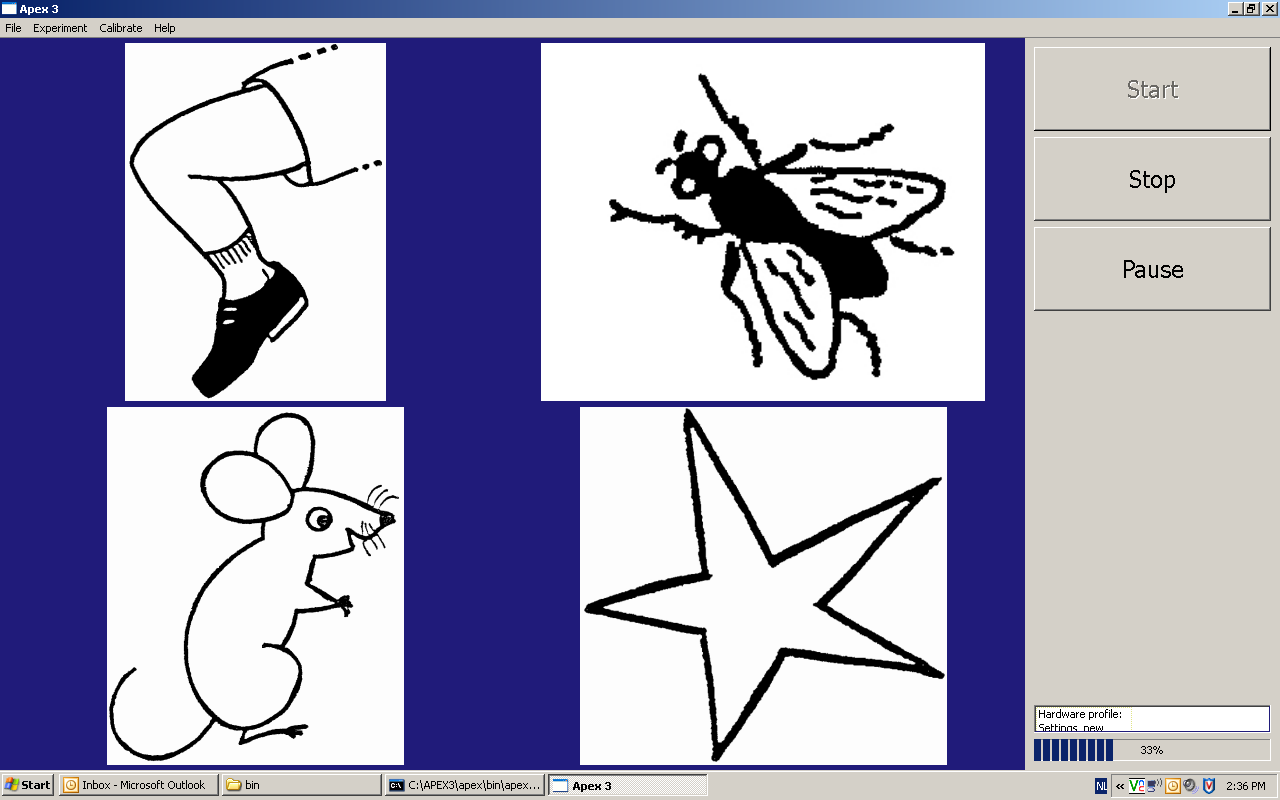
\includegraphics[width=\textwidth]{example1closedset.png}
 \caption{Example of closed-set identification experiment}
 \label{fig:closedset}
\end{figure}

\subsection{Conceptual}
The experiment as described in the previous paragraph should first
be translated to concepts understood by \apex. The main concepts
in this example are \textbf{datablock}, \textbf{stimulus},
\textbf{screen} and \textbf{procedure}. For each of the 3 words to
be presented to the subject, a wave file is available on disk. For
each wave file, a datablock is defined, and for each resulting
datablock a stimulus is defined. Everything that is defined is
assigned an ID, to be able to refer to it later on. Therefore, now
we have 3 stimuli with IDs \id{stimulus_star}, \id{stimulus_mouse}
and \id{stimulus_fly}.

We should also define the things to be shown on the screen during
the experiment. This is done by defining a screen for each word.
Each screen contains 4 pictures, of which one corresponds to the
word. Each screen again gets an ID, in this case we name the
screen by the pictures it contains. Therefore we now have 3
screens with ID \id{screenstar_horse_vase_moon},
\id{screenknee_fly_mouse_star} and \id{screenmouse_fly_star_moon}.

To indicate the order in which the words should be presented, and
together with which screen, a procedure is defined. In the
procedure a number of trials is defined. Recall that a trial is
the combination of a screen, a stimulus and a correct answer.
Therefore a trial is a way to link each of our stimuli with a
screen.

Now only the output logic remains to be defined. The idea is to
continuously present a noise signal and to set the level of the
words such that a certain SNR is obtained. To achieve this, we
define 2 filters, the first one is a generator (i.e., a filter
without input channels) that will generate the noise signal. The
other one is an amplifier, which will amplify or attenuate the
words to obtain the desired SNR.

In the following sections each of the elements of the \xml{XML}
file necessary to implement the latter concepts will be described
in detail. The first one is \element {procedure}.

\subsection{Detailed description of various elements}
\begin{lstlisting}
  <procedure xsi:type="apex:constantProcedureType">
    <parameters>
      <presentations>1</presentations>
      <order>sequential</order>
    </parameters>
    <trials>
      <trial id="trial_star">
        <answer>picturestar</answer>
        <screen id="screenstar_horse_vase_moon"/>
        <stimulus id="stimulus_star"/>
      </trial>
      <trial id="trial_fly">
        <answer>picturefly</answer>
        <screen id="screenknee_fly_mouse_star"/>
        <stimulus id="stimulus_fly"/>
      </trial>
      <trial id="trial_mouse">
        <answer>picturemouse</answer>
        <screen id="screenmouse_fly_star_moon"/>
        <stimulus id="stimulus_mouse"/>
      </trial>
    </trials>
  </procedure>
\end{lstlisting}

The attribute \xml{xsi:type="apex:constantProcedureType"}
indicates that a constant stimuli procedure is used. This means
that the procedure will select the next trial from the trial list
and that it completes after every trial has been presented a
certain number of times.
\begin{itemize}

\item \element{parameters} defines the behavior of the procedure
\begin{itemize}

\item \element{presentations} every trial is presented once

\item \element{order} \xml{sequential} the three trials are
presented sequentially, in the order that is specified in the
experiment file
\end{itemize}
\index{presentations} \index{order}

\item \element{trials} contains different \element{trial} elements
to specify a trial. After selecting a trial the
\element{procedure} will show the specified screen and send the
stimulus to the device. Each trial is given an ID (arbitrary
name), eg \id{TrialStar}, such that it can be referred to later on
or viewed in the results file.

\item \element{answer} the correct answer, to be used by \apex to
determine whether the subject's response is correct. Here, the
subject gets the opportunity to click on one of 4 pictures. The
result from the screen (the subject's response) will be the ID of
the element of the screen that was clicked. Therefore, in this
example, we specify the ID of the picture corresponding to the
stimulus that is presented.
\end{itemize}

A trial must be defined for all the words of the experiment.

\index{trial} \index{answer} \index{screen} \index{stimulus}

\begin{lstlisting}
    <corrector xsi:type="apex:isequal"/>
\end{lstlisting}
\index{corrector}

The corrector checks whether the response is correct or not. The
attribute \xml{xsi:type="apex:isequal"} compares whether the two
input values are exactly the same. In this example
\element{corrector} compares the answer specified under trial and
the ID corresponding to the picture that has been clicked.

\begin{lstlisting}
<screens>
    <uri_prefix>closedset</uri_prefix>
    <reinforcement>
      <progressbar>true</progressbar>
      <feedback length="600">false</feedback>
    </reinforcement>
    <screen id="screenstar_horse_vase_moon">
      <gridLayout height="2" width="2">
        <picture id="picturestar" row="1" col="1">
          <path>star.jpg</path>
        </picture>
        <picture id="picturehorse" row="2" col="1">
          <path>horse.jpg</path>
        </picture>
        <picture id="picturevase" row="1" col="2">
          <path>vase.jpg</path>
        </picture>
        <picture id="picturemoon" row="2" col="2">
          <path>moon.jpg</path>
        </picture>
            </gridLayout>
      <buttongroup id="buttongroup1">
        <button id="picturestar"/>
        <button id="picturehorse"/>
        <button id="picturevase"/>
        <button id="picturemoon"/>
                </buttongroup>
      <default_answer_element>buttongroup1</default_answer_element>
    </screen>
    <screen id="screenknee_fly_mouse_star">
      <gridLayout height="2" width="2">
        <picture id="pictureknee" row="1" col="1">
          <path>knee.jpg</path>
        </picture>
        <picture id="picturefly" row="2" col="1">
          <path>fly.jpg</path>
        </picture>
        <picture id="picturemouse" row="1" col="2">
          <path>mouse.jpg</path>
        </picture>
        <picture id="picturestar" row="2" col="2">
          <path>star.jpg</path>
        </picture>
      </gridLayout>
      <buttongroup id="buttongroup2">
        <button id="pictureknee"/>
        <button id="picturefly"/>
        <button id="picturemouse"/>
        <button id="picturestar"/>
      </buttongroup>
      <default_answer_element>buttongroup2</default_answer_element>
    </screen>
    <screen id="screenmouse_fly_star_moon">
      <gridLayout height="2" width="2">
        <picture id="picturemouse" row="1" col="1">
          <path>mouse.jpg</path>
        </picture>
        <picture id="picturefly" row="2" col="1">
          <path>fly.jpg</path>
        </picture>
        <picture id="picturestar" row="1" col="2">
          <path>star.jpg</path>
        </picture>
        <picture id="picturemoon" row="2" col="2">
          <path>moon.jpg</path>
        </picture>
      </gridLayout>
      <buttongroup id="buttongroup3">
        <button id="picturemouse"/>
        <button id="picturefly"/>
        <button id="picturestar"/>
        <button id="picturemoon"/>
      </buttongroup>
      <default_answer_element>buttongroup3</default_answer_element>
    </screen>
  </screens>
\end{lstlisting}

\element{screens} contains several \element{screen} elements that
can be referred to elsewhere in the experiment file (e.g., in
\element{procedure} above).

\begin{itemize}
\item \element{uri_prefix} a relative path is specified here
(relative with respect to the experiment file). Since \apex knows
the location of the experiment file, only the folder containing
the wave files and pictures must be specified. It is also possible
to give the absolute path, starting at the root. There are 3 ways
to specify a prefix: by directly specifying an absolute path, by
directly specifying a path relative to the experiment file or by
referring to a prefix stored in \filename{apexconfig.xml}. Please
refer to section~\ref{sec:prefixes} for more information.

\item \element{reinforcement} includes

\begin{itemize}

\item \element{progressbar} As the value is \xml{true} a
progressbar will be displayed in the right hand bottom corner of
the screen that indicates how many trials have been completed and
how many remain.

\item \element{feedback length} duration of time after response
(in msec) that \apex waits before presenting the next trial.
During this interval, feedback can be displayed. In this case, no
feedback (thumb up, thumb down) is given as the value is
\xml{false}.

\end{itemize}
\end{itemize}

\begin{itemize}
\item \element{screen} For each word to be presented, a screen is
defined. Each screen has an ID by which it can be referred to
elsewhere in the experiment file (e.g. in \element{trials} to
associate it with a stimulus).
\begin{itemize}

\item \element{gridLayout} specifies how the four figures will be
arranged on the screen. A GridLayout creates a regular grid on the
screen with the specified number of rows and columns. In this
example there are 2 rows and 2 columns. Each figure is defined by
means of a \element{picture} element. Such a definition can be
seen as associating a graphics file with an ID and specifying at
what position of the layout it should be shown. In this case, jpeg
files are used, but other formats are also possible (e.g., png,
bmp, gif).

\begin{itemize}
\item \element{picture}


\element{uri} since the prefix as specified under
\element{uri_prefix} is preprended to each \element {uri}  it
suffices to give the name of the .jpeg file in \element{path}. The
path is relative to the experiment file.

\end{itemize}
\end{itemize}
\begin{itemize}
\item \element{buttongroup} defines a group of screen elements,
namely those (four figures) that are displayed on the screen. The
ID is defined before.

\item \element{default_answer_element} As many elements can be
defined in a screen, \apex has no way to know which element
contains the subject's response. If, for example, a text box is
shown and 2 buttons, it is unclear which is to be used to
determine whether the answer is correct or not. Therefore, in
\element{default_answer_element} the element is designated that
contains the subject's response. In the case of screen elements
that are clicked in order to respond, the example is further
complicated by the fact that we cannot specify just one of the
elements (buttons, pictures), but the response rather comes from a
group of elements. This is when a \element{buttongroup} can be
used to group together different screen elements.
\end{itemize}
\end{itemize}
\index{screens} \index{uri prefix} \index{reinforcement}
\index{progressbar} \index{feedback length} \index{screen}
\index{gridlayout} \index{picture} \index{path}
\index{buttongroup} \index{default answer element}

In this example 5 datablocks are defined, 3 for the word files, 1
for the noise and 1 for silence.

\begin{lstlisting}
 <datablocks>
    <uri_prefix>closedset/</uri_prefix>
    <datablock id="datablock_star">
      <device>wavdevice</device>
      <uri>star.wav</uri>
    </datablock>
    <datablock id="datablock_fly">
      <device>wavdevice</device>
      <uri>fly.wav</uri>
    </datablock>
    <datablock id="datablock_mouse">
      <device>wavdevice</device>
      <uri>mouse.wav</uri>
    </datablock>
    <datablock id="noisedata">
      <device>wavdevice</device>
      <uri>noise.wav</uri>
    </datablock>
    <datablock id="silence">
      <device>wavdevice</device>
      <uri>silence:500</uri>
    </datablock>
  </datablocks>
\end{lstlisting}
\index{datablocks}

\element{datablocks} contains 5 \element{datablock} elements and a
prefix.
\begin{itemize}
\item \element{uri_prefix} a relative path is specified here. It
is also possible to give the absolute path, starting at the root
(see section~\ref{sec:prefixes}).

\item \element{datablock} For each wave file a datablock is made,
with an ID.  \item Each datablock is associated to a
\element{device} (by means of the ID of the device). In datablock
\id{silence} the special syntax is demonstrated for creating a
datablock containing only silence (i.e., all samples are zeros).
This is done to prevent the speech and noise from starting at the
same time. The length of the silence datablock is specified in ms
after the prefix \xml{silence}. It is added before the signal, not
before the noise.

\end{itemize}
\index{datablocks} \index{uri prefix} \index{datablock}
\index{device} \index{uri}

A datablock must be made for all wave files used in the
experiment, including the noise (that will be used by the noise
generator).



In the next sections, the output logic will be defined.
Figure~\ref{fig:ex1-output} gives an overview of the building
blocks that are used in this example. On the left hand side the
datablocks are shown. In the middle the noise generator and the
amplifier and on the right hand side the sound card. As the words
are to be amplified or attenuated according to the desired SNR,
the corresponding datablocks are routed through the amplifier.

\begin{figure}
 \centering
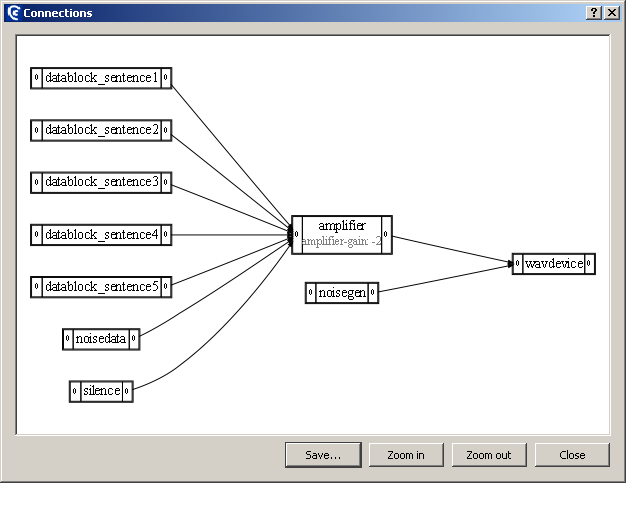
\includegraphics[width=0.5\textwidth]{connectionswindow.png}
 \caption{The connection window}
 \label{fig:ex1-output}
\end{figure}

In the next element the output device is specified.

\begin{lstlisting}
 <devices>
    <device id="wavdevice" xsi:type="apex:wavDeviceType">
      <driver>portaudio</driver>
      <card>default</card>
      <channels>1</channels>
      <samplerate>44100</samplerate>
    </device>
  </devices>

\end{lstlisting}
\index{devices}

All devices defined in the experiment file are grouped in
\element{devices}. In this example there is only 1
\element{device} element. Its ID is set to \id{soundcard}. As an
ID is unique for an entire experiment file, it can be used later
on to refer to this device.

\begin{itemize}
\item  The \xml{xsi:type="apex:wavDeviceType"} attribute tells
\apex that a sound card is used. The experiment only starts if all
devices can be opened.

\item \element{driver} specifies the software driver to be used
for sound output. If unsure, set it to \xml{portaudio}.

\item \element{card} specifies the name of the sound card to be
used. The system default card can be used by specifying
\xml{default} as a card name. Other card names can be defined in
\filename{apexconfig}.

\item \element{channels} specifies the number of channels of the
sound card to be used. The number of channels is restricted to the
selected sound card, with a maximum of 2 for portaudio.

\item \element{samplerate} the sampling rate of the sound card;
Not all sampling rates are supported by all devices, and some
drivers automatically convert the sampling rate. Check your sound
card documentation. The sample rate of the sound card should
correspond to the sampling rates of all datablocks used with it.
If not, an error message will be shown.

\end{itemize}

\index{device} \index{driver} \index{card} \index{channels}
\index{gain} \index{samplerate}

Filters must be defined whenever the signal (or noise) is
manipulated. In this example the level of the noise remains
constant and the signal is amplified or attenuated using an
amplifier filter (loop of \element{datablock}).

\begin{lstlisting}
<filters>
    <filter xsi:type="apex:dataloop" id="noisegen"> (*@\label{xml:filter1}@*)
      <device>wavdevice</device>
      <channels>1</channels>
      <continuous>false</continuous>
      <datablock>noisedata</datablock>
      <basegain>-5</basegain>
      <gain id="noisegain">0</gain>
      <randomjump>true</randomjump>
    </filter>
    <filter xsi:type="apex:amplifier" id="amplifier">  (*@\label{xml:filter2}@*)
      <device>wavdevice</device>
      <channels>1</channels>
      <basegain>-5</basegain>
      <gain id="gain">0</gain>
    </filter>
  </filters>
\end{lstlisting}
\index{filter}

\element{filters} contains individual \element{filter} elements,
which specify a filter, or as a special case a generator (i.e., a
filter without input channels).
\begin{itemize}

\item \element{filter} on line~\ref{xml:filter1} the attribute
\xml{xsi:type="apex:dataloop"} tells \apex that a dataloop
generator has to be created. This is a generator that takes a
datablock and loops it infinitely. The datablock to be looped is
specified by its ID \id{noisedata}. The dataloop generator itself
is assigned the ID \id{noisegen}.


\item \element{filter} on line~\ref{xml:filter2} the attribute
\xml{xsi:type="apex:amplifier"} tells \apex that an amplifier is
to be created. The gain of this amplifier will be varied to change
the amplitude of the words and thus the SNR. It is assigned ID
\id{amplifier}. The gain of the amplifier is made a variable
parameter by assigning it ID \id{gain}
\begin{itemize}
\item \element{device} The device with which the filter is
associated \item \element{channels} The number of channels of the
filter. The available number of channels is dependent on the type
of filter. An amplifier can have any number of channels.

\item If \element{continuous} is set to \xml{true}, the filter or generator
will keep on running in between two trials (i.e., when the subject is responding).
 In this example it stops when the stimulus stops playing (\xml{false}).

\item \element{datablock} The datablock with ID noisedata,
specified under \element{datablocks} will be looped.

\item \element{basegain} the total gain of the amplifier is
basegain+gain. Basegain cannot be a parameter, gain can be a
parameter. The total gain of the complete output system should not
be larger than 0 to avoid clipping of the signal. This is why
basegain = -5.

\item \element{gain} extent to which the signal is amplified.

\item If \element{randomjump} is set to \xml{true}, when the dataloop is started, it will jump to a random sample in the datablock. Thereafter it is looped.
\end{itemize}
\end{itemize}

\index{filters} \index{filter} \index{device} \index{channels}
\index{continuous} \index{datablock} \index{basegain} \index{gain}
\index{randomjump}

\begin{lstlisting}
<stimuli>
    <stimulus id="stimulus_star">
      <datablocks>
        <sequential>
          <datablock id="silence"/>
          <datablock id="datablock_star"/>
          <datablock id="silence"/>
        </sequential>
      </datablocks>
    </stimulus>
    <stimulus id="stimulus_fly">
      <datablocks>
        <sequential>
          <datablock id="silence"/>
          <datablock id="datablock_fly"/>
          <datablock id="silence"/>
        </sequential>
      </datablocks>
    </stimulus>
    <stimulus id="stimulus_mouse">
      <datablocks>
        <sequential>
          <datablock id="silence"/>
          <datablock id="datablock_mouse"/>
          <datablock id="silence"/>
        </sequential>
      </datablocks>
    </stimulus>
  </stimuli>
\end{lstlisting}
\index{stimuli} \index{datablocks}


\element{stimuli} contains different \element{stimulus}, each with
an ID \element{stimulus}

\begin{itemize}\item \element{datablocks}
can be combined in \element{sequential} order (as opposed to
\element{simultaneous}.
\end{itemize}

This is repeated for all the stimuli in the experiment.

\index{stimuli} \index{stimulus} \index{datablocks}
\index{sequential}

\begin{lstlisting}
<connections>
    <connection>
      <from>
        <id>_ALL_</id>
        <channel>0</channel>
      </from>
      <to>
        <id>amplifier</id>
        <channel>0</channel>
      </to>
    </connection>
    <connection>                (*@\label{xml:cha}@*)
      <from>
        <id>amplifier</id>
        <channel>0</channel>
      </from>
      <to>
        <id>wavdevice</id>
        <channel>0</channel>
      </to>
    </connection>               (*@\label{xml:chb}@*)
    <connection>                (*@\label{xml:chc}@*)
      <from>
        <id>noisegen</id>
        <channel>0</channel>
      </from>
      <to>
        <id>wavdevice</id>
        <channel>0</channel>
      </to>
    </connection>               (*@\label{xml:chd}@*)
  </connections>

\end{lstlisting}
\index{connections}

\index{channel}

\element{connections} defines how the different datablocks and
filters are routed to the output device. The ID \id{_ALL_} stands
for all the datablocks. In this example they are routed to the
first channel of the filter with ID {amplifier} (defined under
\element{filters}). In the amplifier the signal is amplified or
attenuated and sent to the wavdevice on lines~\ref{xml:cha}
to~\ref{xml:chb}. At the same time the noise, generated by a
generator with ID noisegen, is sent to the same channel of the
wavdevice. The channels are numbered from 0 onwards. The level of
the noise remains constant and does not pass through an amplifier
(lines~\ref{xml:chc} to~\ref{xml:chd}).

A visual representation of connections can be obtained by choosing
``Show stimulus connections'' under ``Experiment''in the main
\apex menu (top left menu bar).



\begin{lstlisting}
<results>
   <xsltscript>idn.xsl</xsltscript>
</results>
\end{lstlisting}

Even if \element{results} is not specified in the experiment file
\apex will deliver a results file in XML.
\begin{itemize}
\item \element{xsltscript}  a script can transform the XML data to
an easier readable format; this script can be stored in folder
\filename{scripts} under \apex. For more information please read
section~\ref{sec:Using XSLT transforms}.
\end{itemize}
\index{results} \index{xsltscript}

\begin{lstlisting}
<interactive>
   <entry type="int" description="SNR in dB"
    expression="/apex:apex/filters/filter[@id='amplifier']/gain"
    default="0"/>
 </interactive>
\end{lstlisting}

If a small part of an experiment file has to be changed right
before the start of an experiment (e.g. a start value, a gain
value, the subject's name), \apex can show the experimenter a
small \ac{gui} containing the elements to be changed. This is
accomplished by defining the \element{interactive} element in the
experiment file.

In this example we will modify the gain of the filter with ID
\id{amplifier} to a value that is entered by the experimenter at
the start of the experiment.

It is only possible to change the value of an existing element of the experiment file, elements cannot be added. For each element to be changed, an \element{entry} should be defined under \element{interactive}. \element{entry} has  four attributes that should be defined:

\begin{itemize}
\item \attribute{type} specifies the type of input element that
will be shown. If it is \xml{int}, a spinbox\footnote{A spinbox is
an input field that only accepts numbers and has 2 buttons to
respectively increase or decrease its value} will be shown. If it
is \xml{string} a plain text box will be shown. In this case a
spinbox will be shown as a gain is always numeric. \item
\attribute{description} defines the text to be shown in the
\ac{gui} next to the input element, such that the experimenter
knows exactly what to fill in. \item \attribute{expression}
defines the element of the experiment file to be changed. It is
specified by a so-called XPath expression \footnote{see
\url{http://www.w3.org/TR/xpath}}. For a description of XPath, we
refer to the according standard or a good XML book.

\oxygen{OxygenXML can generate XPath expressions for you. First
point the cursor to the target element, then click the right mouse
button and select. An XPath expression to the clicked location is
now in the clipboard and can be pasted at the appropriate place
using the paste function.} \item \attribute{default} specifies the
default value to be shown in the input element.
\end{itemize}

\index{interactive} \index{entry type} \index{expression}

\begin{lstlisting}
<general>
    <showresults>true</showresults>
    <saveprocessedresults>true</saveprocessedresults>
</general>
\end{lstlisting}

\element{general} defines some general parameters. Saving
processed results in a results file is only possible if a
XSLT-script is defined. See section~\ref{sec:Using XSLT
transforms}.

\begin{itemize}
\item \element{showresults} If \xml {true} a window will appear
after completion of the experiment asking whether the results
should be shown on screen.

\item \element{saveprocessedresults} If \xml {true} the
experimenter will be asked whether the processed results must be
appended to the results file.
\end{itemize}

\index{general} \index{showresults} \index{saveprocessedresults}

\newpage
\section{Example 2: Identification of speech in noise using an adaptive method}

\subsection{General description of the experiment}
See \filename{examples/manual/sentenceinnoise.apx}. This is an
example of an adaptive speech in noise test. It determines the
 \ac{srt}, the 50 percent correct point, using
the 1-down, 1-up method described by \citet{PM79}. In this
adaptive procedure the first sentence is repeated with increasing
level until it is identified correctly. Subsequently, the SRT is
determined by increasing or decreasing the level in steps of 2 dB,
according to the last response. Other decision procedures (eg
2-down 1-up) can also be implemented using \apex. In this example
the 5 sentences are scored on the basis of their keywords. The
keywords are indicated in bold on the screen. The
experimenter/clinician is seated in front of the screen and
decides whether the subject has repeated the keywords (of the
sentence) correctly, after which the correct or incorrect button
is clicked(figure~\ref{fig:sentencenoise}). No feedback is
provided. The starting level is given in signal-to noise ratio
(the level of the noise remains the same, that of the signal
varies). In this example speech and noise are routed to the same
channel, i.e. one speaker or one earpiece of the headphone. The
results are written to a results file.

\begin{figure}
 \centering
 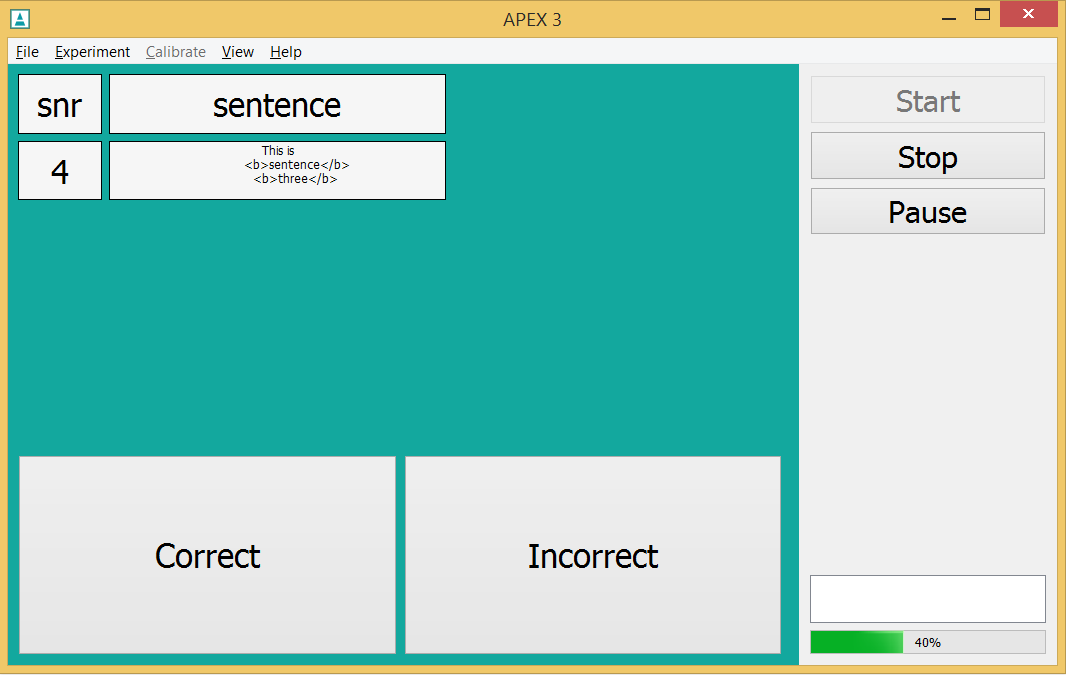
\includegraphics[width=\textwidth]{example2sentenceinnoise.png}
 \caption{Example of adaptive sentence in noise experiment}
 \label{fig:sentencenoise} \todo{bold werkt niet correct?}

\end{figure}
\subsection{Conceptual}
The experiment as described in the previous paragraph should first
be translated to concepts understood by \apex. The main concepts
in this example are \textbf{datablock}, \textbf{stimulus},
\textbf{screen}, \textbf{procedure}, a \textbf{variable} parameter
(to change the gain) and \textbf{fixed Parameter} to show a
sentence on the screen. For each sentence a datablock is defined,
and for each resulting datablock a stimulus is defined. As always,
everything that is defined, is assigned an ID, to be able to refer
to it later on. In this example there are 5 stimuli with IDs
\id{stimulus_sentence1}, \id{stimulus_sentence2},
\id{stimulus_sentence3}, \id{stimulus_sentence4} and
\id{stimulus_sentence5}. The procedure defines a number of trials.
Recall that a trial is the combination of a screen (always the
same in this example), a stimulus and a response.

As we are dealing with an adaptive procedure a fixed or variable
parameter is adapted. In this example a variable parameter is
adapted to change the gain of the sentence, and a fixed parameter
is used to show a sentence on the screen. The screen also shows
the signal-to-noise ratio (SNR) under test and the response
alternatives ``correct'' and ``incorrect''.

Now only the output logic remains to be defined. The idea is to
continuously present a noise signal and to vary the level of the
sentences adaptively. To achieve this, we define 2 filters, the
first one is a generator (i.e., a filter without input channels)
that will generate the noise signal. The other one is an
amplifier, which will amplify or attenuate the sentences to obtain
the desired SNR. Both are connected to one channel of the
wavdevice.

In the following sections each of the elements of the XML file
necessary to implement the latter concepts will be described in
detail.

\subsection{Detailed description of various elements}

\begin{lstlisting}
<procedure xsi:type="apex:adaptiveProcedure">
  <parameters>
    <presentations>1</presentations>
    <order>sequential</order>
    <corrector xsi:type="apex:isequal"/>
    <nUp>1</nUp>
    <nDown>1</nDown>
    <adapt_parameter>gain</adapt_parameter>
    <start_value>0</start_value>
    <stop_after_type>presentations</stop_after_type>
    <stop_after>1</stop_after>
    <larger_is_easier>true</larger_is_easier>
    <repeat_first_until_correct>true</repeat_first_until_correct>
    <stepsizes><stepsize begin="0" size="2"/></stepsizes>
  </parameters>

  <trials>
    <trial id="trial_sentence1">
         <answer>button_correct</answer>
         <screen id="screen"/>
         <stimulus id="stimulus_sentence1"/>
    </trial>

    <trial id="trial_sentence2">
         <answer>button_correct</answer>
         <screen id="screen"/>
         <stimulus id="stimulus_sentence2"/>
    </trial>

    <trial id="trial_sentence3">
        <answer>button_correct</answer>
        <screen id="screen"/>
        <stimulus id="stimulus_sentence3"/>
    </trial>

    <trial id="trial_sentence4">
        <answer>button_correct</answer>
        <screen id="screen"/>
        <stimulus id="stimulus_sentence4"/>
    </trial>

    <trial id="trial_sentence5">
        <answer>button_correct</answer>
        <screen id="screen"/>
        <stimulus id="stimulus_sentence5"/>
    </trial>
  </trials>
</procedure>
\end{lstlisting}


The attribute \xml{xsi:type="adaptiveProcedureType"} of
\element{procedure} refers to a procedure in which a parameter is
changed according to the response of the subject. In this example
the gain of the amplifier is adapted. The procedure selects the
next trial from the trial list and it completes after every trial
has been presented a certain number of times.

\begin{itemize}
\item \element{parameters} defines the behavior of the procedure

\begin{itemize}

\item \element{presentations} every trial is presented once

\item \element{order} the trials are presented sequentially, in
the order that is specified in the experiment file (if
\xml{random} would be specified, they would be presented in random
order).

\item \element{corrector} the corrector checks whether the response is correct or not. The
attribute \xml{xsi:type="apex:isequal"} compares whether the two
input values are exactly the same. In this example
\element{corrector} compares the answer specified under trial  (\id{button_correct}) and
the ID corresponding to the picture that has been clicked (either \id{button_correct} or \id{button_incorrect}).

\item \element{nUp} the level is increased after n (here 1)
incorrect response(s); cf \element{larger_is_easier}

\item \element{nDown} the level is decreased after n (here 1)
correct response(s); cf \element{larger_is_easier}

\item \element{adapt_parameter} to be adapted

\item \element{start_value} the experiment starts with gain=0
(input of user). The value here will be replaced by the entry
value. Please refer to section~\ref{sec:Interactive} for more
information.

\item \element{stop_after_type} the experiment stops after a
specified number of presentations of each trial is completed (it
is also possible to stop after \element{reversals}.

\item \element{stop_after} the experiment stops after 1
presentation of each trial

\item \element{larger_is_easier} If \xml{true}, then larger values
of the parameter are easier than smaller values. It is used to
determine \element{nUp} and \element{nDown}.

\item \element{repeat_first_until_correct} the first trial is
repeated with increasing gain until it is identified correctly.

\item \element{stepsizes} from the beginning of the experiment
(begin=0) the stepsize is 2 dB.
\end{itemize}

\item \element{trials} contains different \element{trial} elements
to specify a trial. Once a trial is selected, \element{procedure}
will show the specified screen and send the stimulus to the
device. Each trial is given an ID (arbitrary name), eg
\id{trialsentence1}, such that it can be referred to later on or
viewed in the results file. A trial must be defined for all the
sentences of the experiment.

\item \element{answer} the correct answer, to be used by \apex to
determine whether the subject's response is correct. In this
example the experimenter will click on ``correct'' or
``incorrect''. The result from the screen will be the ID of the
element of the screen that was clicked (\id{button_correct} or
\id{button_incorrect}).

\end{itemize}

\index{parameters}

\index{procedure}

\index{presentations}

\index{order}

\index{corrector}

\index{nUp}

\index{nDown}

\index{adapt parameter}

\index{start value}

\index{stop after type}

\index{stop after}

\index{larger is easier}

\index{repeat first until}

\index{stepsizes}

\index{trial}

\index{answer}

\begin{lstlisting}
<screens>
        <reinforcement>
            <progressbar>true</progressbar>
            <feedback length="600">false</feedback>
        </reinforcement>

        <screen id="screen">
       <gridLayout height="2" width="1" id="main_layout" rowstretch="1,2">
               <gridLayout width="4" height="4" columnstretch="1,4,2,2"
               rowstretch="1,1,2,2" id="parameter_layout" row="1" col="1">

    <label id="snrlabel" row="1" col="1">
    <text>snr</text>
    </label>

    <parameterlabel id="snr" row="2" col="1">
      <parameter>gain</parameter>
    </parameterlabel>

    <label id="sentence" row="1" col="2">
    <text>sentence</text>
    </label>

    <parameterlabel id="sentence" row="2" col="2">
    <fontsize>12</fontsize>
    <parameter>sentence</parameter>
    </parameterlabel>

    </gridLayout>

    <gridLayout height="1" width="2" id="answer_layout" x="1" y="2">
    <button x="1" y="1" id="button_correct">
    <text>Correct</text>
     </button>
    <button x="2" y="1" id="button_wrong">
    <text>Incorrect</text>
    </button>

    </gridLayout>
    </gridLayout>
    <buttongroup id="buttongroup">
    <button id="button_correct"/>
    <button id="button_wrong"/>
    </buttongroup>
    <default_answer_element>buttongroup</default_answer_element>
    </screen>
    </screens>>
\end{lstlisting}

\element{screens} contains \element{screen} element that is
referred to in \element{procedure}.

\begin{itemize}
\item \element{reinforcement} includes elements on progress and
feedback
\begin{itemize}

\item \element{progressbar} If the value is \xml {true} a progress
bar will be displayed in the right hand bottom corner of the
screen that indicates the percentage of trials that have been completed.

\item \element{feedback length} duration of the time after
response (in msec) that \apex waits before presenting the next
trial. During this interval feedback can be displayed. In this
example, no feedback (thumb up, thumb down) is given as the value
is \xml{false}.
\end{itemize}

\item \element{screen} the screen has an ID by which it can be
referred to in each trial. In this example the screen displays
four blocks in the top left corner to indicate the SNR and the
sentence. In addition, the labels ``Correct'' and ``Incorrect''
are displayed on the buttons at the bottom of the screen (cfr
screenshot, figure...).
\begin{itemize}

\item \element{gridlayout} places elements in an irregular grid.
The screen is divided into sections according to the values. In
this example there are two nested layouts. The main layout divides the screen in two main rows (height = 2, width = 1).
The parameter layout divides the first of these rows in four rows and four columns, of which only the two first ones are filled.
The answer layout divides the second main row in two columns, each with one button.
The stretch factor for the columns is a list of integers, separated by
comma's. There should be as many integers as columns. The width of
the columns is proportional to the numbers. With \xml{width="1"},
and \xml{height="2"} \xml{rowstretch="1,2"} implies that the
second row will be twice as wide as the first one. If
\xml{width="4"}, and \xml{height="4"} and
\xml{columnstretch="1,4,2,2"} the second column will be four times
as wide as the first and two times as wide as the 3rd and 4th.
With \xml{columnstretch="1,1,2,2"} the 3rd and 4th rows will be
twice as wide as the 1st and 2nd.

\item \element{label} the labels on the left are fixed and display
the \element{text} ``SNR'' and ``Sentence''. The button
``Correct'' and ``Incorrect'' are indicated at the bottom of the
screen

\item \element{parameterlabel} the blocks on the right display the values
of the fixed parameters. Gain is the (variable) SNR level, and
sentence is a fixed parameter, defined in \element{stimulus}

\item \element{font size} can be specified in points

\item \element{buttongroup} defines a group of screen elements
(those that are displayed on the screen). As many elements can be
defined in a screen, \apex has no way to know which element
contains the subject's response. Therefore, in
\element{default_answer_element} the element is designated that
contains the subject's response. In the case of screen elements
that are clicked in order to respond, the example is further
complicated by the fact that we cannot specify just one of the
elements (one button, one picture), but that the response rather comes
from a group of elements. This is when a \element{buttongroup} can
be used to group together different screen elements.


\end{itemize}
\end{itemize}
\index{screens} \index{reinforcement} \index{progressbar}
\index{feedback} \index{screen} \index{gridlayout} \index{label}
\index{parameter label} \index{font size} \index{buttongroup}
\index{default answer element}

\begin{lstlisting}
<datablocks>
  <uri_prefix>sentences/</uri_prefix>
  <datablock id="datablock_sentence1">
    <device>wavdevice</device>
    <uri>sent1.wav</uri>
  </datablock>
  <datablock id="datablock_sentence2">
    <device>wavdevice</device>
    <uri>sent2.wav</uri>
  </datablock>
  <datablock id="datablock_sentence3">
    <device>wavdevice</device>
    <uri>sent3.wav</uri>
  </datablock>
  <datablock id="datablock_sentence4">
    <device>wavdevice</device>
    <uri>sent4.wav</uri>
  </datablock>
  <datablock id="datablock_sentence5">
    <device>wavdevice</device>
    <uri>sent5.wav</uri>
  </datablock>
  <datablock id="noisedata">
    <device>wavdevice</device>
    <uri>noise.wav</uri>
  </datablock>
  <datablock id="silence">
    <device>wavdevice</device>
    <uri>silence:500</uri>
  </datablock>
</datablocks>
\end{lstlisting}


\element{datablocks} contains a list of \element{datablock}
elements and a prefix.
\begin{itemize}
\item \element{uri_prefix} a relative path is specified here
(relative with respect to the experiment file). Since \apex knows
the location of the experiment file, only the folder containing
the wave files and pictures must be specified. It is also possible
to give the absolute path, starting at the root. There are 3 ways
to specify a prefix: by directly specifying an absolute path, by
directly specifying a path relative to the experiment file or by
referring to a prefix stored in \filename{apexconfig.xml}. Please
refer to section~\ref{sec:prefixes} for more information. \todo{necessary to repeat all this information here, not enough to refer to prefixes section? (Lot)}

\item \element{datablock} for each wave file a datablock is made,
with an ID.

In datablock \id{silence} the special syntax is
demonstrated for creating a datablock containing only silence
(i.e., zeros). This is done to put silence before and after the
sentence, to prevent the speech and noise from
starting at the same time. The length of the silence datablock is
specified in ms after the prefix \xml{silence}. It is added before the signal (in element \element{stimulus}), not
before the noise.

\begin{itemize}
\item the datablock is associated with the sound card with ID
\id{wavdevice}, as defined in the \element{devices} section.

\item \element{uri} the URI is appended to the prefix defined
above

\end{itemize}
\end{itemize}
\index{uri prefix}

\index{datablocks}

\index{datablock}

\index{device}

\index{uri}


\begin{lstlisting}
<devices>
    <device id="wavdevice" xsi:type="apex:wavDeviceType">
    <driver>portaudio</driver>
    <card>default</card>
    <channels>1</channels>
    <samplerate>44100</samplerate>
    </device>
</devices>
\end{lstlisting}

All devices defined in the experiment file are grouped in
\element{devices}.The ID is set to \id{wavdevice}. As an ID is
unique for an entire experiment file, it can be used later on to
refer to this device (eg in datablocks).

\begin{itemize}
\item \element{device} the \xml{xsi:type="apex:wavDeviceType"}
attribute tells \apex that a sound card is used. The experiment
only starts if all devices can be opened.

\item \element{driver} specifies the software driver to be used
for sound output. If unsure, set it to \xml{portaudio}.

\item \element{card} specifies the name of the sound card to be
used. The system default card can be used by specifying
\xml{default} as a card name. Other card names can be defined in
\filename{apexconfig.xml}.

\item \element{samplerate} the sampling frequency of the sound
card. Not all sampling rates are supported by all devices, and
some drivers automatically convert the sampling rate. Check your
sound card documentation. The sample rate of the sound card should
correspond to the sampling rates of all \element{datablocks} used
with it.
\end{itemize}

\index{device} \index{driver} \index{card} \index{channels}
\index{gain} \index{samplerate}

\begin{lstlisting}
<filters>
<filter xsi:type="apex:dataloop" id="noisegen">
    <device>wavdevice</device>
    <channels>1</channels>
    <continuous>false</continuous>
    <datablock>noisedata</datablock>
    <basegain>-5</basegain>
    <gain>0</gain>
    <randomjump>true</randomjump>
    </filter>
<filter xsi:type="apex:amplifier" id="amplifier" >
    <device>wavdevice</device>
    <channels>1</channels>
    <basegain>-5</basegain>
    <gain id="gain">0</gain>
</filter>
</filters>
\end{lstlisting}

\element{filters} contains individual \element{filter} elements,
which specify a filter, or as a special case a generator (i.e., a
filter without input channels).

\begin{itemize}

\item The attribute \xml{xsi:type="apex:dataloop"} tells \apex
that a dataloop generator has to be created. This is a generator
that takes a datablock and loops it infinitely. The datablock to
be looped is specified by its ID \id {noisedata}.

\item \element{filter} on line~\ref{xml:filter2} the attribute
\xml{xsi:type="apex:amplifier"} tells \apex that an amplifier has
to be created. The gain of this amplifier will be varied to change
the amplitude of the words and thus the SNR. It is assigned ID
\id{amplifier}. The gain of the amplifier is made a variable
parameter by assigning it ID \id{gain}

\begin{itemize}

\item \element{device} the device with which the filter is
associated

\item \element{channels} The number of channels of the filter. The
available number of channels depends on the type of filter. An
amplifier can have any number of channels.

\item \element{continuous} If set to \xml{false} the noise is
presented during the speech, but not during the subject's
response.

\item \element{datablock} the datablock with ID noisedata,
specified under \element{datablocks} will be looped.

\item \element{basegain}:  the total gain of the amplifier is
basegain+gain. The total gain of the complete output system should
not be larger than 0 to avoid clipping of the signal. This is why
basegain = -5.

\item \element{gain} the gain value that is changed. E.g. if the
targetamplitude is 65 dB SPL (see Calibration) the signal and
noise have equal amplitude if gain = 0. Gain is changed by other
modules.

\item If \element{randomjump} is set to \xml{true}, when the
dataloop is started, it will jump to a random sample in the
datablock. Thereafter it is looped.

\end{itemize}

\end{itemize}
\index{filters} \index{filter} \index{device} \index{channels}
\index{continuous} \index{datablock} \index{basegain} \index{gain}
\index{randomjump}

\begin{lstlisting}
<stimuli>
  <fixed_parameters>
    <parameter id="sentence"/>
  </fixed_parameters>

  <stimulus id="stimulus_sentence1">
    <datablocks>
    <sequential>
        <datablock id="silence"/>
        <datablock id="datablock_sentence1"/>
        <datablock id="silence"/>
    </sequential>
    </datablocks>

  <fixedParameters>
    <parameter id="sentence">This is <b> sentence </b> <b>one</b></parameter>
  </fixedParameters>
  </stimulus>

  <stimulus id="stimulus_sentence2">
    <datablocks>
    <sequential>
        <datablock id="silence"/>
        <datablock id="datablock_sentence2"/>
        <datablock id="silence"/>
    </sequential>
    </datablocks>

  <fixedParameters>
    <parameter id="sentence">This is <b> sentence </b> <b>two</b></parameter>
    </fixedParameters> </stimulus>

  <stimulus id="stimulus_sentence3">
    <datablocks>
    <sequential>
        <datablock id="silence"/>
        <datablock id="datablock_sentence3"/>
        <datablock id="silence"/>
    </sequential>
    </datablocks>

<fixedParameters>
<parameter id="sentence">This is <b> sentence </b> <b>three</b></parameter>
</fixedParameters>
</stimulus>

<stimulus id="stimulus_sentence4">
    <datablocks>
    <sequential>
        <datablock id="silence"/>
        <datablock id="datablock_sentence4"/>
        <datablock id="silence"/>
    </sequential>
    </datablocks>

<fixedParameters>
<parameter id="sentence">This is <b> sentence </b> <b>four</b></parameter>
</fixedParameters>
</stimulus>

<stimulus id="stimulus_sentence5">
    <datablocks>
    <sequential>
        <datablock id="silence"/>
        <datablock id="datablock_sentence5"/>
        <datablock id="silence"/>
    </sequential>
    </datablocks>

   <fixedParameters> <parameter id="sentence">This is <b> sentence
   </b> <b>five</b> </parameter> </fixedParameters> </stimulus>
</stimuli>
\end{lstlisting}

\element{stimuli} contains different \element{stimulus}, each with
an ID.

\begin{itemize}
\item \element{fixedParameters} is used here to be able to show
the sentence under test on the Screen. Fixed parameters are
discussed in section~\ref{sec:Parameters}.


\begin{itemize}
\item \element {parameter} the fixed parameter is defined here and
should also be defined in each \element {stimulus}
\end{itemize}

\item \element{stimulus} Each stimulus gets an ID (referred to in
\element {trial})
\begin{itemize}

\item \element{datablocks} here one refers to the
\element{datablock} described before; it includes the sentence
file.

\begin{itemize}
\item \element{sequential} The sequence of \element{datablocks} is
indicated here.
\end{itemize}

\item \element{fixedParameters} sets the fixed parameter for each
\element{stimulus}.

\item \element{b} indicates which words (the keywords) should
appear in bold on screen.
\end{itemize}
\end{itemize}

This is repeated for all the sentences.

\index{stimuli}

\index{fixed parameters}

\index{stimulus}

\index{datablocks}

\index{sequential}

\index{parameter}



\begin{lstlisting}
<connections>
    <connection>
        <from>
        <id>_ALL_</id>
        <channel>0</channel>
        </from>
        <to>
        <id>amplifier</id>
        <channel>0</channel>
        </to>
    </connection>
    <connection>                (*@\label{xml:ch1}@*)
        <from>
        <id>amplifier</id>
        <channel>0</channel>
        </from>
        <to>
        <id>wavdevice</id>
        <channel>0</channel>
        </to>
    </connection>               (*@\label{xml:ch2}@*)
    <connection>                (*@\label{xml:ch3}@*)
        <from>
        <id>noisegen</id>
        <channel>0</channel>
        </from>
        <to>
        <id>wavdevice</id>
        <channel>0</channel>
        </to>
        </connection>           (*@\label{xml:ch4}@*)
</connections>
\end{lstlisting}

\index{connections} \index{channel}

\begin{itemize}
\item \element{connections} defines how the different datablocks
and filters are routed to the output device. The ID \id{_ALL_}
stands for all the datablocks. In this example they are routed to
the first channel of the filter with ID {amplifier} (defined under
\element{filters}). In the amplifier the signal is amplified or
attenuated and sent to the wavdevice on lines~\ref{xml:ch1}
to~\ref{xml:ch2}. At the same time the noise, generated by a
generator with ID noisegen, is sent to the same channel of the
wavdevice. The channels are numbered from 0 onwards. The level of
the noise remains constant and does not pass through an amplifier
(lines~\ref{xml:ch3} to ~\ref{xml:ch4}). Although noisedata is a
\element{datablock} and connected to \emph{amplifier} it is not
specified in \element{stimulus} and does not pass through
\emph{amplifier}.
\end{itemize}

A visual representation of connections can be obtained by choosing
``Show stimulus connections'' under ``Experiment''in the main
\apex menu (top left menu bar).


\begin{lstlisting}
 <results>
  <page>apex:resultsviewer.html</page>
  <resultparameters>
   <parameter name="reversals for mean">4</parameter>
  </resultparameters>
  <showduringexperiment>false</showduringexperiment>
  <showafterexperiment>true</showafterexperiment>
  <saveprocessedresults>true</saveprocessedresults>
 </results>
\end{lstlisting}


\element{results} Even if \element{results} is not specified in
the experiment file \apex will save a results file in XML.

\todo{new part, to check!}
\begin{itemize} 
\item \element{page} URL of the html page to show in the results window. The page should have the appropriate java script methods embedded. More example pages can be found in the \apex resultsviewer folder.
\item \element{resultparameters} Parameters to be passed to the results page. Each parameter will be set in hash params. In this example, the result will be calculated as the mean of the variable parameter (gap) at the last 4 reversals.  \todo{what is hash params? (lot)}
\item \element{showduringexperiment} If true, an extra window will be created which will show the results of the current experiment while the experiment is being executed. Javascript embedded in the page will be executed upon each new trial.
\item \element{showafterexperiment} If true, when the experiment is finished, a dialog box will appear querying whether results should be shown. If the answer is affirmative, a new window will be opened and the results will be shown after javascript processing.
\item \element{saveprocessedresults} If \xml {true} the
experimenter will be asked whether the processed results must be
appended to the results file. This will only work if the results are successfully saved to disk and your javascript code supports this transformation.
\end{itemize}

\index{results} \index{page} \index{resultparameters} \index{showduringexperiment} \index{showafterexperiment} \index{saveprocessedresults}


\begin{lstlisting}
<interactive> <entry type="int" description="SNR start value"
  expression="/apex:apex/procedure/parameters/start_value" default="4" />
</interactive>
\end{lstlisting}

If a small part of an experiment file has to be changed right
before the start of an experiment (e.g. a start value, a gain
value, the subject's name), \apex can show the experimenter a
small \ac{gui} containing the elements to be changed. This is
accomplished by defining the \element{interactive} element in the
experiment file.

In this example we will modify the gain of the filter with ID
\id{amplifier} to a value that is entered by the experimenter at
the start of the experiment.

\begin{itemize}
\item \element{entry type} a value is entered, here corresponding
to SNR in dB. It is also possible to enter a string, e.g. name of
the subject (see Reference Manual).

\item \element{expression} the interactive window will show 4 as
default value; more than one entry may be defined.
\end{itemize}

\index{interactive}

\index{entry type}

\index{expression}

\newpage
\section{Example 3: Gap detection: determining the Just Noticeable Difference}

\todo{example needs modifications, corrector and choices = outdated? modified own version to create new figure }

\subsection{General description of the experiment}
See \filename{examples/manual/gapdetection.apx}. This is an
example of a gap detection task: two stimuli are presented to the
listener in random order, a stationary noise and an interrupted
noise. During the presentation the intervals are highlighted. The
subject's task is to indicate the interval with the
interruption(figure~\ref{fig:gapdetection}). Feedback is provided
(thumb up, thumb down) and the minimal detectable gap is
determined by means of an adaptive procedure (here 2-down, 1-up).
Stimuli (wave files) are generated off line. This example only
includes 5 wave files. Usually many more are generated. The
results are written to a text file.


\begin{figure}
 \centering
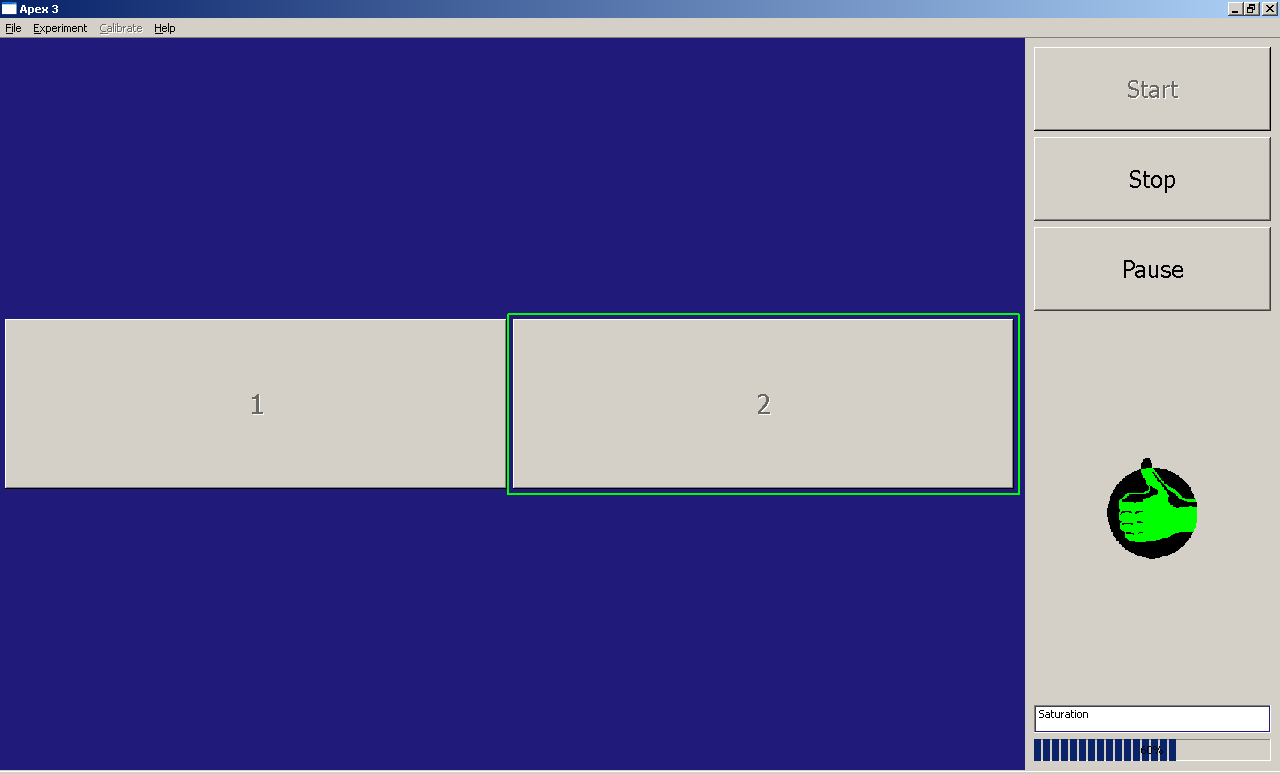
\includegraphics[width=\textwidth]{example3gapdetection.png}
 \caption{Example of adaptive gap detection experiment}
 \label{fig:gapdetection}
\end{figure}

\subsection{Conceptual}
The experiment as described in the previous paragraph should first
be translated to concepts understood by \apex. The main concepts
used here are \textbf{procedure}, \textbf{screens},
\textbf{datablocks} and \textbf{stimuli}.

For each wave file (noise with or without a gap) a \element
{datablocks} is defined, and for each datablock a \element
{stimulus} is defined. In this example there are 5 wave files,
with gap sizes ranging between 1 and 5 ms. Their IDs are
\id{g5ms}, \id{g4ms}, \id{g3ms},\id{g2ms} and \id{g1ms}. In an
adaptive procedure either a fixed or variable parameter is
defined. In this example a fixed parameter is used, i.e. the gap
size in the stimulus. The wave files with different gap sizes are
stored on disk, and are assigned a certain gap value. This gap
value is used to determine the gap threshold. Also, a \element
{screen} is defined that shows the two response intervals
indicating ``1'' and ``2''.

To indicate the order in which the stimuli should be presented a
\element {procedure} is defined. An adaptive procedure is defined
containing 1 \element {trial} with five variable stimuli (with
gap) and the standard stimulus without the gap. Recall that a
\element {trial} is the combination of a \element {screen} (always
the same in this example), a stimulus and a correct answer. The
standard and stimuli occur randomly in one of both intervals.

Now only the output logic remains to be defined. The idea is to
present the standard and a variable stimulus after each other, and
the stimulus to be presented depends on the response of the
subject. Filters are not used since the signals are not changed.

In the following sections each of the elements of the XML file
necessary to implement the latter concepts will be described in
detail.

\subsection{Detailed description of various elements}

\todo{modifications: to check, corrector?}
\begin{lstlisting} 
<procedure xsi:type="apex:adaptiveProcedure">
   <parameters>
     <presentations>1</presentations>
     <order>sequential</order>
     <intervals count="2">
	<interval number="1" element="button1"/>
	<interval number="2" element="button2"/>
	</intervals>
     <pause_between_stimuli>1000</pause_between_stimuli>
     <nUp>1</nUp>
     <nDown>2</nDown>
     <adapt_parameter>gap</adapt_parameter>
     <start_value>5</start_value>
     <stop_after_type>reversals</stop_after_type>
     <stop_after>5</stop_after>
     <min_value>0</min_value>
     <max_value>5</max_value>
     <larger_is_easier>true</larger_is_easier>
     <stepsizes>
       <change_after>reversals</change_after>
       <stepsize  begin="0" size="2"/>
       <stepsize begin="2" size="1"/>
     </stepsizes>
  </parameters>

  <trials>
    <trial id="trial1" >
     <screen id="screen1" />
     <stimulus id="stimulus1" />
     <stimulus id="stimulus2"/>
     <stimulus id="stimulus3"/>
     <stimulus id="stimulus4"/>
     <stimulus id="stimulus5"/>
     <standard id="standard"/>
    </trial>
  </trials>
</procedure>
\end{lstlisting}


\element{procedure} The attribute
\xml{xsi:type="adaptiveProcedureType"} refers to a procedure in which a parameter is changed according to
the response of the subject. In this example 1 trial is defined
with different stimuli from which the adaptive procedure chooses.

\begin{itemize}
\item \element{parameters} defines the behavior of the procedure
(eg., nr of presentations, order of presentation, response
strategy).

\begin{itemize}
\item \element{presentation} every trial is presented once.

\item \element{order} applies to the order of the trials. Since there is only 1
\element{trial}, it does not matter here wether the order is
specified as \element{sequential} or \element{random}.

\item \element{corrector} the corrector checks whether the
response is correct or not. In this example the number of choices
in \element{procedure} was 2. This means that \element{procedure}
will present the target stimulus in either interval 1 or 2.
\element{procedure} informs \element{corrector} about the correct
interval. \element{Corrector} also receives the clicked button from the
screen and looks up the corresponding number in the
\element{interval} element above and compares it with the number it
received from \element{procedure}. \todo{check}

\item \element{alternatives} number of alternatives to choose from
(here: 2 intervals) and the IDs of the buttons (defined under \element{screens} they correspond to.

\item \element{pause_between_stimuli} a pause of 1000 ms will be
introduced between successive wave files;

\item \element{nUp} number of items after incorrect trials to
increase the gap

\item \element{nDown} number of items after correct trials to
decrease the gap

\item \element{min_value} the gap size cannot be smaller than 0.

 \item \element{max_value} the gap size cannot be larger than 5

\item \element{adapt_parameter} the parameter to change, here the
``gap'', see also \element{fixed_parameters}

\item \element{start_value} the gap at which to start, here 5, see
under \element{stimulus}

\item \element{stop_after_type} reversals (it can also stop after
a number of presentations or trials)

\item \element{stop_after} number of reversals after which the
procedure is stopped

\item \element{rev_for_mean} the number of reversals that are used
for the average threshold

\item \element{larger_is_easier} here \xml{true} (the smaller the
gap, the more difficult the task)

\item \element{stepsizes} the stepsize

\end{itemize}

\begin{itemize}
\item\element{change_after} the \element{stepsize} is changed
after a specified number of reversals. In this example a stimulus
is skipped until the second reversal (start at 5, then 3, etc).
Thereafter no stimulus is skipped.

\end{itemize}

\item \element{trials} only 1 trial is defined

\begin{itemize}

\item \element{trial} the ID of the trial

\item\element{screen} the ID of the screen

\item \element{stimulus} the ID of the stimulus

\item \element{standard} the ID of the standard

\end{itemize}
\end{itemize}

\index{parameters}

\index{presentation}

\index{order}

\index{corrector}

\index{alternatives}

\index{pause between stimuli}

\index{nUp}

\index{nDown}

\index{adapt parameter}

\index{start value}

\index{stop after type}

\index{min value}

\index{max value}

\index{larger is easier}

\index{stepsize}

\index{trials}

\index{screen}

\index{stimulus}

\index{standard}



\begin{lstlisting}
<screens>
  <reinforcement>
    <progressbar>true</progressbar>
    <feedback length="300">true</feedback>
    <showcurrent>true</showcurrent>
  </reinforcement>

  <screen id="screen1" >
    <gridLayout height="1" width="2" id="main_layout">
      <button x="1" y="1" id="button1" >
       <text>1</text>
      </button>
      <button x="2" y="1" id="button2" >
       <text>2</text>
      </button>
    </gridLayout>
  <buttongroup id="buttongroup1">
     <button id="button1"/>
     <button id="button2"/>
  </buttongroup>
    <default_answer_element>buttongroup1</default_answer_element>
 </screen>
</screens>
\end{lstlisting}

\begin{itemize}
\item \element{screens} contains several screen elements that can
be referred to elsewhere in the experiment file (e.g. in
\element{procedure} above).


\item \element{reinforcement} includes elements on progress and
feedback

\begin{itemize}

\item \element{progressbar} if \xml {true} a progress bar will be
displayed in the right hand bottom corner of the screen. The
progress bar can indicate the percentage of trials that have been done or it
shows when a reversal occurs in an adaptive procedure. In the
latter case the progress bar will increase at every reversal while
the number of trials varies.

\item \element{feedback length} duration of the time after
response (in msec) that \apex waits before presenting the next
trial. During this interval feedback can be displayed.

\item \element{showcurrent} if \xml{true} the interval is highlighted while a
signal is presented.
\end{itemize}

\item \element{screen} each screen has an ID by which it can be
referred to elsewhere in the experiment. In this example the
screen displays two intervals.

\begin{itemize}


\item \element{gridlayout}places elements in an irregular grid.
The screen is divided into sections according to the values. In
this example there is an equal number of rows (x) and columns (y).

Gridlayout defines a group of screen elements (those that are
displayed on the screen).

\begin{itemize}
\item \element{button} for each interval a button is specified;
this button (interval) displays a number on the screen

\item \element{text} the left interval denotes ``1'', the right
one denotes ``2''.

\end{itemize}

\item \element{buttongroup} defines a group of screen elements
(those that are displayed on the screen). As many elements can be
defined in a screen, \apex has no way to know which element
contains the subject's response. Therefore, in
\element{default_answer_element} the element is designated that
contains the subject's response. In the case of screen elements
that are clicked in order to respond, the example is further
complicated by the fact that we cannot specify just one of the
elements (one button, one picture), but that the response rather comes
from a group of elements. This is when a \element{buttongroup} can
be used to group together different screen elements.

\end{itemize}
\end{itemize}



\index{screens}

\index{reinforcement}

\index{progressbar}

\index{feedback length}

\index{showcurrent}

\index{screen}

\index{gridlayout}

\index{button}

\index{text}

\index{buttongroup}

\index{default answer element}

\begin{lstlisting}
<datablocks>
  <uri_prefix>Gapfiles</uri_prefix>
    <datablock id="g5ms" >
      <device>wavdevice</device>
      <uri>g5.wav</uri>
    </datablock>

    <datablock id="g4ms" >
      <device>wavdevice</device>
      <uri>g4.wav</uri>
    </datablock>

    <datablock id="g3ms"  >
      <device>wavdevice</device>
      <uri>g3.wav</uri>
    </datablock>

    <datablock id="g2ms" >
      <device>wavdevice</device>
      <uri>g2.wav</uri>
    </datablock>

    <datablock id="g1ms"  >
      <device>wavdevice</device>
      <uri>g1.wav</uri>
    </datablock>

    <datablock id="datablockref">
      <device>wavdevice</device>
      <uri>ref500.wav</uri>
    </datablock>
  </datablocks>
\end{lstlisting}


\element{datablocks} contains a list of \element{datablock}
elements and a prefix.

\begin{itemize}
\item \element{uri_prefix}: a relative path is specified here.
Since \apex knows the location of the experiment file, only the
folder containing the wave files and pictures must be specified.



\item \element{datablock} for each wave file a unique datablock is
defined by an ID. The standard signal (uninterrupted noise) must
also be specified here.

\item \element{device} each datablock includes the audio device to
which the signal is routed

\item \element{uri} since the path is defined in
\element{uri_prefix} it is not necessary to specify the entire
path again

\index{datablocks} \index{uri prefix} \index{datablock}
\index{device} \index{uri}

\end{itemize}
\begin{lstlisting}
<devices>
 <device id="wavdevice" xsi:type="apex:wavDeviceType">
 <driver>portaudio</driver>
 <card>default</card>
 <channels>2</channels>
 <gain>0</gain>
 <samplerate>44100</samplerate>
 </device>
</devices>
\end{lstlisting}


\element{devices} all devices defined in the experiment file are
grouped in the \element{devices}. Only 1 \element{device} is used
in this example. The ID is set to soundcard. As an ID is unique
for an entire experiment file, it can be used later on to refer to
this device.

\begin{itemize}
\item \element{device} the \xml{xsi:type="apex:wavDeviceType"}
attribute tells \apex that a sound card is used. The experiment
only starts if all devices can be opened.

\item \element{driver} specifies the software driver to be used
for sound output. If unsure, set it to \xml{portaudio}.

\item \element{card} specifies the name of the sound card to be
used. The system default card can be used by specifying
\xml{default} as a card name. Other card names can be defined in
ApexConfig.

\item \element{channels} 2 channels are specified here, because
the signal is stereo.

\item \element{samplerate} the sampling frequency of the wave
files. Not all sampling rates are supported by all devices, and
some drivers automatically convert the sampling rate. Check your
sound card documentation. The sample rate of the sound card should
correspond to the sampling rates of all datablocks used with it.

\end{itemize}

\index{devices}

\index{driver}

\index{card}

\index{channels}

\index{gain}

\index{samplerate}


\begin{lstlisting}
<stimuli>
   <fixed_parameters>
     <parameter id="gap"/>
   </fixed_parameters>

   <stimulus id="stimulus1" >
     <description>noisewithgap1</description>
     <datablocks>
       <datablock id="g5ms" />
     </datablocks>
     <fixedParameters>
       <parameter id="gap">5</parameter>
     </fixedParameters>
   </stimulus>

   <stimulus id="stimulus2" >
     <description>noisewithgap2</description>
     <datablocks>
       <datablock id="g4ms" />
     </datablocks>
       <fixedParameters>
        <parameter id="gap">4</parameter>
     </fixedParameters>
   </stimulus>

   <stimulus id="stimulus3" >
     <description>noisewithgap3</description>
     <datablocks>
       <datablock id="g3ms" />
     </datablocks>
      <fixedParameters>
       <parameter id="gap">3</parameter>
      </fixedParameters>
   </stimulus>

   <stimulus id="stimulus4" >
     <description>noisewithgap4</description>
     <datablocks>
       <datablock id="g2ms" />
     </datablocks>
       <fixedParameters>
        <parameter id="gap">2</parameter>
       </fixedParameters>
   </stimulus>

   <stimulus id="stimulus5" >
     <description>noisewithgap5</description>
     <datablocks>
       <datablock id="g1ms" />
     </datablocks>
       <fixedParameters>
         <parameter id="gap">1</parameter>
       </fixedParameters>
   </stimulus>

   <stimulus id="standard">
     <datablocks>
      <datablock id="datablockref"/>
     </datablocks>
       <fixedParameters>
        <parameter id="gap">0</parameter>
     </fixedParameters>
   </stimulus>
</stimuli>
\end{lstlisting}


\element{stimuli} defines the auditory events, e.g. noise with gap
and noise without gap.

\begin{itemize}

\item \element{fixedParameters}

\begin{itemize}
\item \element{parameter} the gap is a fixed parameter that is
identified by an ID
\end{itemize}

\item \element{stimulus} this element includes a description of
the (variable) stimulus

\begin{itemize}
\item \element{description}

\item \element{datablocks} the ID refers to the wave file corresponding to the datablock

\item \element{fixedParameter}
\begin{itemize}
\item \element{parameter} includes information on the size of the
variable gap
\end{itemize}

\end{itemize}
\end{itemize}


\index{stimuli}

\index{fixed parameters}

\index{stimulus}

\index{datablocks}

\index{parameter}

\index{standard}

\begin{lstlisting}
<connections>
   <connection>
     <from>
       <id>_ALL_</id>
       <channel>0</channel>
     </from>
     <to>
       <id>wavdevice</id>
       <channel>1</channel>
     </to>
   </connection>

 </connections>
\end{lstlisting}

\index{connections} \index{channel}

\begin{itemize}
\item \element{connections} defines how the different datablocks
and filters are routed to the output device. The ID \id{_ALL_}
stands for all the datablocks. In this example they are routed to
1 channel of the wavdevice.
\end{itemize}

A visual representation of connections can be obtained by choosing
``Show stimulus connections'' under ``Experiment''in the main
\apex menu (top left menu bar).


\begin{lstlisting}
<results>
  <page>apex:resultsviewer.html</page>
  <resultparameters>
   <parameter name="reversals for mean">3</parameter>
  </resultparameters>
  <showduringexperiment>false</showduringexperiment>
  <showafterexperiment>true</showafterexperiment>
  <saveprocessedresults>true</saveprocessedresults>
 </results>
\end{lstlisting}

\element{results} Even if \element{results} is not specified in
the experiment file \apex will save a results file in XML. The results file
will display the correct answers, the reversals, the entire
sequence of responses, and the average threshold based on the
number of reversals and the magnitude of the corresponding gap
parameter specified in the experiment file.

\todo{new part, to check!}
\begin{itemize} 
\item \element{page} URL of the html page to show in the results window. The page should have the appropriate java script methods embedded. More example pages can be found in the \apex resultsviewer folder.
\item \element{resultparameters} Parameters to be passed to the results page. Each parameter will be set in hash params. \todo{perhaps some moren explanation on what this can be and why it is empty here?}
\item \element{showduringexperiment} If \xml{true}, an extra window will be created which will show the results of the current experiment while the experiment is being executed. Javascript embedded in the page will be executed upon each new trial.
\item \element{showafterexperiment} If \xml{true}, when the experiment is finished, a dialog box will appear querying whether results should be shown. If the answer is affirmative, a new window will be opened and the results will be shown after javascript processing.
\item \element{saveprocessedresults} If \xml{true} the
experimenter will be asked whether the processed results must be
appended to the results file. This will only work if the results are successfully saved to disk and your javascript code supports this transformation.
\end{itemize}

\index{results} \index{page} \index{resultparameters} \index{showduringexperiment} \index{showafterexperiment} \index{saveprocessedresults}



\begin{lstlisting}
 <general>
  <exitafter>true</exitafter>
 </general>
\end{lstlisting}

\element{general} defines some general parameters.

\begin{itemize}
\item \element{exitafter} if \xml{true} \apex will close after the experiment has ended and results have been shown.
\end{itemize}

\newpage
\section{Example 4: Gap detection in child mode}

\subsection{General description of the experiment}
See \filename{examples/manual/gapdetectionchild.apx}. This is an
example of a gap detection task adapted to the interest of
children: two stimuli are presented to the listener in random
order, a stationary noise and an interrupted noise. It is the same
experiment as example 3, but pictures (movies) of cars replace
buttons on the screen, and a smiley panel is
shown(figure~\ref{fig:gapchild}). During the presentation of
stimuli the cars are animated. The child's task is to indicate the
stimulus with the interruption. Feedback is provided by smileys
and the minimal detectable gap is determined by means of an
adaptive procedure (here 2-down, 1-up). Only those elements that
are specific to the child mode are described in this example.

\index{Example: gap detection - child mode}

\begin{figure}
 \centering
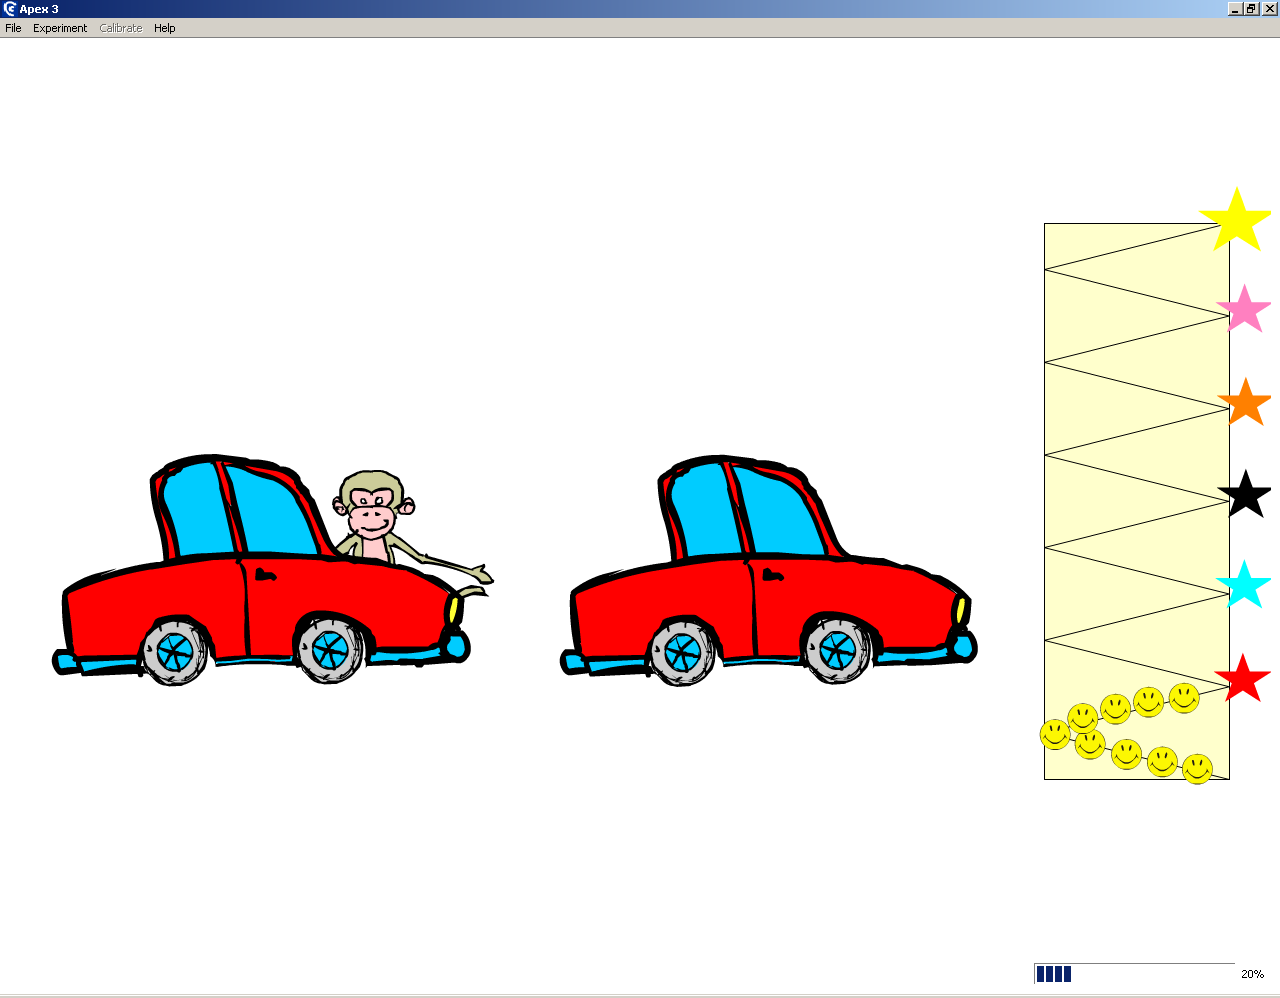
\includegraphics[width=\textwidth]{example4gapdetectionchild.png}
 \caption{Example of gap detection in child mode}
 \label{fig:gapchild}
\end{figure}

\subsection{Conceptual}
The main concepts illustrated in this example are
\textbf{childmode}, and \textbf{reinforcement}. Child mode
involves a different panel, and intro/outro movies.

\subsection{Detailed description of various elements}

\begin{lstlisting}
<screens>
    <uri_prefix>car/</uri_prefix>
    <general>
      <showpanel>true</showpanel>
    </general>
    <reinforcement>
      <progressbar>true</progressbar>
      <feedback length="300">true</feedback>
      <showcurrent>true</showcurrent>
    </reinforcement>
    <childmode>
      <panel>reinforcement.swf</panel>
    </childmode>
    <screen id="screen1">
      <gridLayout height="1" width="2" id="main_layout">
        <flash row="1" col="1" id="button1">
          <path>stillcar.swf</path>
          <feedback>
            <highlight>rijden.swf</highlight>
            <positive>goodcar.swf</positive>
            <negative>badcar.swf</negative>
          </feedback>
        </flash>

        <flash row="1" col="2" id="button2">
          <path>stillcar.swf</path>
          <feedback>
            <highlight>rijden.swf</highlight>
            <positive>goodcar.swf</positive>
            <negative>badcar.swf</negative>
          </feedback>
        </flash>
      </gridLayout>

      <buttongroup id="buttongroup1">
        <button id="button1"/>
        <button id="button2"/>
      </buttongroup>
      <default_answer_element>buttongroup1</default_answer_element>
    </screen>
  </screens>
\end{lstlisting}

\element{screens}

\begin{itemize}
\item \element{uri_prefix} a relative path is specified here
(relative with respect to the experiment file). This only applies
to the movies in \element{screen}. There are 3 ways to specify a
prefix: by directly specifying an absolute path, by directly
specifying a path relative to the experiment file or by referring
to a prefix stored in \filename{apexconfig.xml}. Please refer to
section~\ref{sec:prefixes} for more information.

\item \element{general}

\begin{itemize}

\item \element{show panel} if \xml {true} a panel will be shown
with smileys (see figure \textbf{presented above})

\end{itemize}

\item \element{reinforcement}
\begin{itemize}
\item \element{progressbar} If \xml {true} a progress bar will be
displayed on the right hand side with smileys. The progress bar
shows when a reversal occurs in an adaptive procedure (while the
number of trials varies).

\item \element{feedback length} duration of the time after
response (in msec) that \apex waits before presenting the next
trial. During this interval feedback can be displayed

\item \element{showcurrent} the interval is highlighted while a
signal is presented

\end{itemize}

\item\element{childmode} replaces the ``standard'' panel, sets
some defaults, enables intro/outro movies and changes the
background colour

\begin{itemize}

\item \element{panel} the name of the movie file, per frame
(smileys and panel are a collection of frames)

\end{itemize}

\end{itemize}

\element{screen} Each screen has an ID by which it can be referred
to elsewhere in the experiment. In this example the screen
displays two movies, each containing a car.

\begin{itemize}
\item \element{gridlayout} places elements in an irregular grid.
The screen is divided into sections according to the values. In
this example there are equal number of rows and columns.

\begin{itemize}
\item \element{flash} replaces \element{button} of the standard
version

\begin{itemize}
\item \element{path} the name of the flash movie file on disk,
when there is no animation.

\item \element{feedback}


\item \element{highlight}the name of the file while the car moves

\item \element{positive} the name of the movie file following a
correct response (here a monkey waving)

\item \element{negative} the name of the movie file following an
incorrect response  (the trunk of an elephant)

\end{itemize}

\end{itemize}

\item \element{buttongroup} defines a group of screen elements
(those that are displayed on the screen). As many elements can be
defined in a screen, \apex has no way to know which element
contains the subject's response. Therefore, in
\element{default_answer_element} the element is designated that
contains the subject's response. In the case of screen elements
that are clicked in order to respond, the example is further
complicated by the fact that we cannot specify just one of the
elements (buttons, pictures), but that the response rather comes
from a group of elements. This is when a \element{buttongroup} can
be used to group together different screen elements.


\end{itemize}
\index{screens}

\index{uri prefix}

\index{general}

\index{show panel}

\index{reinforcement}

\index{progressbar}

\index{feedback length}

\index{showcurrent}

\index{childmode}

\index{panel}

\index{screen}

\index{gridlayout}

\index{flash row}

\index{path}

\index{feedback}

\index{highlight}

\index{positive}

\index{negative}

\index{button}

\index{buttongroup}

\index{default answer element}

